\documentclass[11pt,a4paper]{article}

\usepackage[T1]{fontenc}
\usepackage[utf8]{inputenc}
\usepackage{newtxtext,newtxmath}
\usepackage[margin=1in]{geometry}
\usepackage{setspace}
\onehalfspacing
\usepackage{amsmath}
\usepackage{graphicx}
\usepackage{booktabs}
\usepackage{float}
\usepackage{multirow}
\usepackage{array}
\usepackage{enumitem}
\usepackage[labelfont=bf,labelsep=period,font=small,figurename=Fig.]{caption}
\usepackage{xcolor}
\usepackage[colorlinks=true,linkcolor=blue!70!black,citecolor=blue!70!black,urlcolor=blue!70!black]{hyperref}

% Section headings: \large bold for sections, \normalsize bold for subsections
\makeatletter
\renewcommand\section{\@startsection{section}{1}{\z@}%
  {-3.5ex \@plus -1ex \@minus -.2ex}{2.3ex \@plus.2ex}{\normalfont\large\bfseries}}
\renewcommand\subsection{\@startsection{subsection}{2}{\z@}%
  {-3.25ex\@plus -1ex \@minus -.2ex}{1.5ex \@plus .2ex}{\normalfont\normalsize\bfseries}}
\renewcommand\paragraph{\@startsection{paragraph}{4}{\z@}%
  {3.25ex \@plus 1ex \@minus .2ex}{-1em}{\normalfont\normalsize\bfseries}}
% Citations print as bare linked numbers (no brackets), as in the original
\renewcommand\@cite[2]{#1\if@tempswa , #2\fi}
\makeatother

% Let large figures/tables sit at the top of a text page, as in the original
\renewcommand{\topfraction}{0.95}
\renewcommand{\bottomfraction}{0.9}
\renewcommand{\textfraction}{0.05}
\renewcommand{\floatpagefraction}{0.8}
\setcounter{topnumber}{3}
\setcounter{totalnumber}{4}

% Names used throughout
\newcommand{\QC}{Q-\textsc{Compass}}
\newcommand{\QCBi}{Q-\textsc{Compass}-\textsc{Bi}}
\newcommand{\NanoG}{\textsc{NanoG1}}

\title{\textbf{Quatrix: An Empirical Evaluation of \QC{} and SAVO\\on Multimodal Sequence Modeling}}
\author{Syed Abdur Rehman Ali\\[2pt]
  {\small Independent Researcher}\\
  {\small\href{https://github.com/Abd0r}{\texttt{github.com/Abd0r}} $\cdot$ ORCID \href{https://orcid.org/0009-0004-6611-2918}{0009-0004-6611-2918}}}
\date{\small April 2026}

\begin{document}
\maketitle

\begin{center}
\textbf{Abstract}
\end{center}

{\small\noindent\looseness=-1
We evaluate \QC{}~\cite{ref1} --- a value-projection-free attention primitive grounded in the reinforcement-learning $Q$-function --- at three parameter scales (57M, 121M, 179M) across four modalities (WikiText-103, MS-COCO captions, LibriSpeech clean-100, MiniGrid 3D navigation). We evaluate the SAVO four-projection variant in which the $V$ projects the state$\odot$action product instead of the raw input. We also evaluate multi-head \QC{} (MH-QC) and report it as a null result. \textbf{Text-LM parity (controlled ablation):} SAVO sits $+12.33 \pm 0.87$ perplexity above the rank-matched transformer at 60m (paired-difference, 4 seeds, $p = 7.6 \times 10^{-4}$). Full-rank standard 8-head MHA at the same training recipe (2 seeds) reaches $257.96 \pm 2.12$ val ppl --- worse than the rank-matched controlled ablation at this 10,000-step budget, despite having $8\times$ more attention-block parameters. SAVO is $+5.79$ ppl above full-rank MHA on val. The same ${\sim}$12-ppl gap to rank-matched holds at 120m and 180m (single seed each). \textbf{Cross-modal non-interference:} at matched 229M-text-token compute, joint four-modality 60m training reaches the same per-text-token loss as text-only training, and the property holds through 180m. \textbf{Out-of-distribution:} the 60m $W_V$-free SAO has a small OOD edge on arxiv and pubmed; the effect does not replicate at 120m or 180m. We report this as a null result on the $W_V$-free OOD-generalisation hypothesis at the scales tested. \textbf{Cross-field demonstration:} the same SAVO block class runs on four computational-oncology tasks --- signature decomposition (cosine 0.975 vs NNLS 0.987, \textit{NNLS higher}), 27-class pan-cancer (top-1 0.517 vs majority 0.087), GDSC2 drug-response (Pearson 0.903; drug-only baseline 0.864), and TCGA 5-year-survival (C-index 0.701; clinical-only ablation 0.708, \textit{clinical-only higher within seed noise}). \textbf{World-model branch:} the world objective trains concurrently with text/vision/audio without breaking the joint training; world MSE drops from 1.125 at initialisation to 0.071 at step 10,000 (${\sim}16\times$ reduction). The predict-mean baseline on the trained 180m StateEncoder is 0.033 in the same encoded-state metric, reflecting MiniGrid-Empty-8x8's low next-state variance --- benchmarking the routing primitive against dedicated world-model architectures on demanding environments (DMLab, Habitat) is out of scope. The unification claim is a structural property of the routing block. \NanoG{} (cancer foundation model with mid-CoT hypothetical simulation, building on \S\ref{sec:7}) is deferred to a subsequent paper.\par}

\section{Introduction}\label{sec:1}

Current multimodal systems implement vision, audio, and text through separately-designed neural encoders: a ViT image branch~\cite{ref2}, a Whisper audio branch~\cite{ref3}, and a GPT-class text decoder~\cite{ref4}, connected via learned projection layers at fusion points. \QC{}~\cite{ref1} replaces the per-modality design with a single sequence-mixing primitive grounded in the reinforcement-learning $Q$-function: the same primitive, differing only in whether a causal mask is applied, is used for all four modalities. Standard attention variants~\hyperlink{cite.ref5}{5}--\hyperlink{cite.ref9}{9} retain the four-projection $QKVO$ structure and are typically optimized as a separate encoder per modality. \QC{} drops the value projection $W_V$ and scores attention via a $Q$-function over learned state/action projections.

This paper is the empirical follow-up to~\cite{ref1}. It introduces two extensions deferred in that work and evaluates them at three parameter scales (57M, 121M, 179M) on four modalities. The central claims are:

\begin{enumerate}[leftmargin=*,labelindent=\parindent,itemsep=0.6ex]
\item \textbf{SAVO closes most of the SAO$\to$QKVO 60m text-LM gap.} The four-projection variant in which the $V$ projects the state$\odot$action product reduces the perplexity gap from 20 ppl to $+12.33 \pm 0.87$ ppl at 60m (4-seed paired-difference vs the rank-matched controlled ablation, $p = 7.6 \times 10^{-4}$). A comparable ${\sim}$11-ppl gap holds at 120m and 180m (single seed each, magnitude consistent with the 60m multi-seed mean).
\item \textbf{Cross-modal non-interference is empirical, not assumed.} At matched text compute, joint four-modality training at 60m reaches the same per-text-token loss as text-only training; the property holds through 180m.
\item \textbf{World-model concurrent with text/vision/audio.} The world objective trains stably alongside the other three modalities (MSE $1.125 \to 0.071$ over the 10,000-step budget); MiniGrid-Empty-8x8's low next-state variance puts the predict-mean baseline (0.033) in the same band as the trained TransitionModel, so the routing primitive's concurrent multimodal capacity --- not world-model dominance --- is what we report.
\item \textbf{Cross-field demonstration.} The same SAVO block class trains on four computational-oncology tasks (signature decomposition, pan-cancer classification, drug-response regression, 5-year survival prediction). Per-task performance ranges from competitive (Phase 3 GDSC drug-response, $r{=}0.903$) to slightly below specialist baselines (Phase 1 NNLS, Phase 4 clinical-only), indicating the routing primitive trains and converges across these domains; per-domain superiority is not claimed.
\end{enumerate}

The work is purely empirical. The architectural primitive and its theoretical justification are established in~\cite{ref1}; here we ask how it behaves at scale across modalities and where the boundaries of its current evaluation lie.

\section{Related Work}\label{sec:2}

\paragraph{Attention variants.} Numerous works modify the attention mechanism while retaining the QKVO four-projection structure: linear attention~\cite{ref6}, sparse attention~\cite{ref7}, FlashAttention~\cite{ref8}, and grouped-query attention~\cite{ref9}. None eliminate $W_V$ as an architectural decision. \QC{}~\cite{ref1} does, grounding the removal in $Q$-function theory; the four-projection variant introduced here (\S\ref{sec:3.1}) reintroduces a $V$, but the $V$ projects the state-action product, not the raw input.

\begin{figure}[H]
\centering
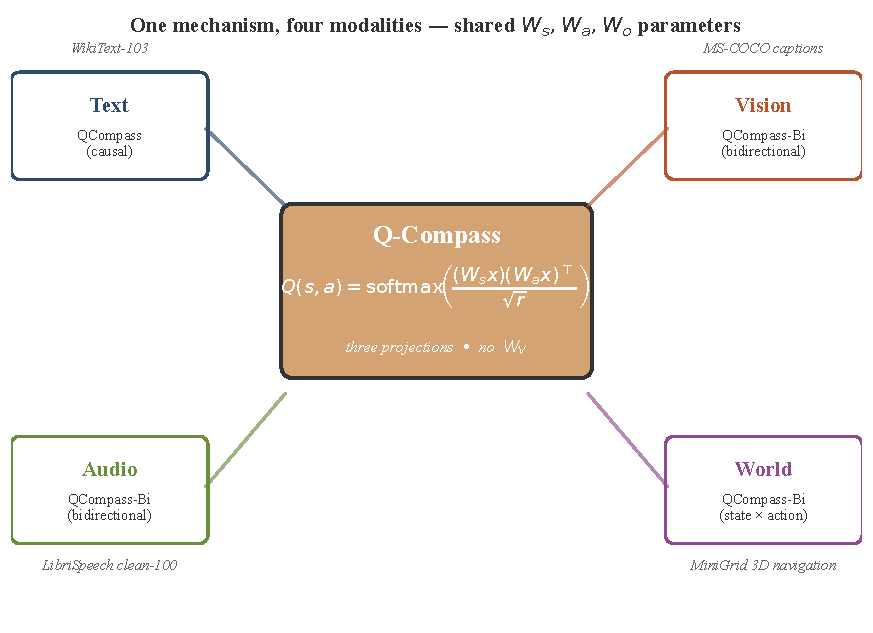
\includegraphics[width=.929\linewidth]{figs/fig01.pdf}
\caption{\textbf{One mechanism, four modalities.} The same \QCBi{} block implements routing for text, vision, audio, and world-model pipelines. Text uses the causal variant (\QC{}); all other modalities use the bidirectional variant (\QCBi{}). The $W_s, W_a, W_o$ projection matrices are structurally identical across pipelines; only dimensionality and layer count vary per modality.}
\label{fig:1}
\end{figure}

\paragraph{Multimodal architectures.} Current systems compose modality-specific encoders: ViT~\cite{ref2} and CLIP~\cite{ref10} for vision; Whisper~\cite{ref3} for audio; GPT-class decoders~\cite{ref4} for text. Flamingo~\cite{ref11} fuses them via learned cross-attention. Perceiver IO~\cite{ref12} introduces a shared latent bottleneck but retains standard attention. Gato~\cite{ref13} tokenizes multiple modalities into a common embedding space for a single transformer decoder; the attention kernel inside Gato is still QKVO, and unification occurs at the tokenization layer rather than at the routing primitive.

\paragraph{World models.} Ha and Schmidhuber~\cite{ref14} and the Dreamer lineage~\cite{ref15} established the state--action--transition decomposition we adopt. We parameterize all three components (StateEncoder, TransitionModel, ActionHead) using \QCBi{} blocks. Our objective here is to test that the routing primitive supports a world-model objective concurrently with text/vision/audio inside a single shared backbone --- not to benchmark against dedicated world-model architectures, for which target-network EMAs, predictor heads, contrastive auxiliaries, and richer environments (DMLab, Habitat) are the standard ingredients.

\section{Method}\label{sec:3}

We use \QC{}~\cite{ref1} as the routing primitive throughout. Given input $x \in \mathbb{R}^{B\times L\times H}$, \QC{} computes $\text{state} = xW_s$, $\text{action} = xW_a$ (both $\in \mathbb{R}^{B\times L\times r}$), $Q(s,a) = \operatorname{softmax}((\text{state}\cdot\text{action}^{\top})/\sqrt{r} + M)$, and $\text{output} = W_o(Q(s,a)\cdot x)$, where $M$ is an optional causal mask. Mechanism, parameter accounting, and the bidirectional variant (\QCBi{}, $M=0$) are described in the original paper. The remainder of this section introduces two architectural variants deferred in~\cite{ref1} and the modality pipelines. Of the two, only SAVO ($W_c$ $Q$-value content) closes the SAO$\to$QKVO text-LM gap; multi-head \QC{} (MH-QC) is a null result we report transparently in \S\ref{sec:5.7}.

\subsection{SAVO: a four-projection \QC{} with $Q$-value content}\label{sec:3.1}

Vanilla \QC{} (the SAO form: state, action, output) gathers raw $x_j$ as content. The SAVO variant replaces this with the token's own self-$Q$-value:
\begin{align}
\text{qval}_i &= \text{state}_i \odot \text{action}_i \qquad \in \mathbb{R}^{r} \label{eq:1}\\
\text{content}_i &= \text{qval}_i \cdot W_c \qquad (W_c \in \mathbb{R}^{r\times H}) \label{eq:2}\\
\text{output} &= W_o\bigl(Q(s,a)\cdot \text{content}\bigr). \label{eq:3}
\end{align}
The semantic reading: each token's content is the $Q$-value signature of itself as an action from its own state, computed from the same projections that drive the routing. Unlike standard attention's $W_V$, $W_c$ projects a $Q$-value (not raw $x$), so the $W_V$-free property of \QC{} is preserved at the principled level. Parameter cost: $+rH$ per block (${\sim}$18K at 60m). Since $\text{state} = xW_s$ and $\text{action} = xW_a$, SAVO's content gather $((xW_s)\odot(xW_a))W_c$ is mathematically a learned non-linear function of $x$. The ``$W_V$-free'' framing applies at the \textit{raw-input} level only --- SAVO is not free of learned content transforms; it replaces a linear projection of $x$ with a non-linear one of $(W_s, W_a, W_c)$ jointly.

\subsection{Multi-head \QC{} (MH-QC)}\label{sec:3.2}

MH-QC splits the state and action projections into $h$ heads of rank $r/h$, computes $Q^{(k)}(s,a)$ in each subspace, and concatenates the outputs:
\begin{equation}
\text{output} = W_o \cdot \bigl[Q^{(1)}\cdot x^{(1)} \,\|\, \cdots \,\|\, Q^{(h)}\cdot x^{(h)}\bigr], \label{eq:4}
\end{equation}
where $x^{(k)}$ is the $k$-th $H/h$ slice of $x$. No additional parameters: $W_s$ and $W_a$ retain their total size $H\times r$. SAVO and MH-QC compose; the combination is denoted MH-QVC. Per-block parameter counts for all four variants are listed in Table~\ref{tab:1}.

\begin{table}[H]
\centering
\small
\setlength{\tabcolsep}{3pt}
\renewcommand{\arraystretch}{1.2}
\begin{tabular*}{\linewidth}{@{\extracolsep{\fill}}lrrr}
\toprule
Variant & Attn-block params (per layer) & 60m ($H{=}384$, $r{=}48$) & 120m ($H{=}640$, $r{=}80$) \\
\midrule
\QC{} single-head (SAO) & $2Hr + H^2$ & 184,320 & 511,600 \\
MH-\QC{} (any $h$) & $2Hr + H^2$ & 184,320 & 511,600 \\
SAVO ($Q$-value content) & $3Hr + H^2$ & 202,752 & 562,800 \\
MH-QVC ($h \geq 1$, with $W_c$) & $3Hr + H^2$ & 202,752 & 562,800 \\
\midrule
Rank-matched transformer (1-head) & $4Hr$ & 73,728 & 204,800 \\
Standard multi-head attention & $4H^2$ & 589,824 & 1,638,400 \\
\bottomrule
\end{tabular*}
\caption{Per-layer attention-block parameter counts (excludes FFN, norms, embeddings). The rank-matched transformer is the apples-to-apples baseline used in \S\ref{sec:5.2}: all four projections at rank $r$, matching \QC{}'s $W_s, W_a$ rank.}
\label{tab:1}
\end{table}

\subsection{Modality pipelines}\label{sec:3.3}

\paragraph{Text (autoregressive LM).} Tokens are embedded via learned token and positional embeddings, passed through $N$ causal \textsc{QuatrixBlocks} (each a \QC{} block plus pre-norm FFN), and projected to vocabulary logits via a tied embedding head. Loss is standard next-token cross-entropy.

\paragraph{Vision.} RGB images ($224\times224$) are patchified via a $16\times16$ Conv2d into 196 patch tokens, position-embedded, passed through 3 bidirectional \QCBi{} blocks, projected to the LM hidden dimension, and prepended to the text token sequence. The joint loss is text cross-entropy over the text portion only; vision tokens do not contribute directly to the loss.

\paragraph{Audio.} Waveforms are loaded at 16\,kHz and converted to 80-mel spectrograms. The spectrogram is treated as a 2D image (frequency $\times$ time) and patchified with a $16\times16$ kernel, producing a variable number of patches. Patches are position-embedded, passed through 3 bidirectional \QCBi{} blocks, projected to the LM hidden dimension, and prepended to the text token sequence.

\paragraph{World.} Frame pairs $(\text{frame}_t, \text{frame}_{t+1})$ from MiniGrid 3D navigation trajectories are encoded via the same \textsc{VisionEncoder} used for vision training. A \textsc{StateEncoder} (a \QCBi{} block with a learnable query token prepended to the patch sequence) aggregates each frame's patches into $s_t$ or $s_{t+1}$. The discrete action ID is embedded into $a_t$. The \textsc{TransitionModel} (9--10 \QCBi{} blocks, taking the fused state-action vector as input) predicts $\hat{s}_{t+1} = \text{Transition}(s_t, a_t)$. World loss is mean squared error with the gradient through the target stopped:
\begin{equation}
\mathcal{L}_{\text{world}} = \text{MSE}\bigl(\hat{s}_{t+1},\ \text{stop\_grad}(s_{t+1})\bigr). \label{eq:5}
\end{equation}
The target detachment prevents trivial collapse via the target pathway. The world objective trains concurrently with the other three modalities; we report convergence and a comparison to the predict-mean baseline in \S\ref{sec:6.3}.

\subsection{Joint training objective and optimization}\label{sec:3.4}

At each step a single batch is sampled from one of four data loaders according to a fixed mixture (35\% text / 25\% vision / 20\% audio / 20\% world). The per-step loss is
\begin{equation}
\mathcal{L}_{\text{total}} = \alpha\,\mathcal{L}_{\text{text}} + \beta\,\mathcal{L}_{\text{vision}} + \gamma\,\mathcal{L}_{\text{audio}} + \delta\,\mathcal{L}_{\text{world}}, \label{eq:6}
\end{equation}
with $\alpha{=}\beta{=}\gamma{=}1.0$ and $\delta{=}0.5$ (world MSE on normalized state vectors has roughly $1/30$ the magnitude of text cross-entropy). We use \textbf{Muon}~\cite{ref16} for 2D linear weight matrices and \textbf{AdamW}~\cite{ref17} for embeddings, LayerNorm, and biases, with separate cosine schedules (peak Muon $3{\times}10^{-4}$, $2.5{\times}10^{-4}$, $2{\times}10^{-4}$ for 60m/120m/180m; AdamW at 1/10). The Muon Newton--Schulz orthogonalisation uses a single-stage schedule with the original~\cite{ref16} coefficients; we did not adopt the V4-style hybrid 8+2-iteration schedule~\cite{ref18} in the runs reported here. The exact iteration coefficients are pinned in the released codebase. Effective batch is 64 sequences of 1024 tokens (batch $4\times$ grad accumulation 16). Training is mixed precision (fp16 compute with loss scaling, fp32 parameters/optimizer), gradient-clipped at $\ell_2$-norm 1.0.

\begin{figure}[H]
\centering
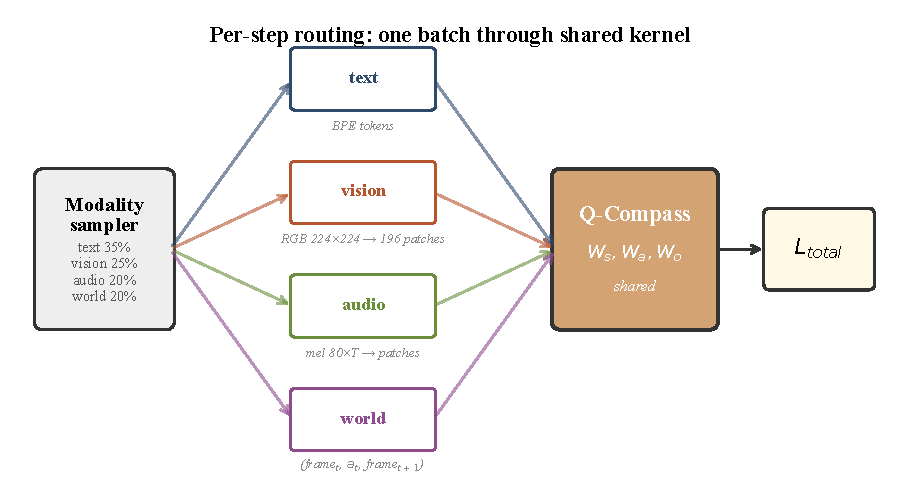
\includegraphics[width=.959\linewidth]{figs/fig02.pdf}
\caption{\textbf{Per-step routing: one batch through the shared kernel.} At each optimizer step the modality sampler draws from text (35\%), vision (25\%), audio (20\%), or world (20\%). Regardless of modality, the batch flows through the same $W_s, W_a, W_o$ parameters inside the \QC{} kernel.}
\label{fig:2}
\end{figure}

\section{Experiment Setup}\label{sec:4}

\paragraph{Datasets.} Text: WikiText-103~\cite{ref19}, 200,000 contiguous samples (min.\ 512-character length) tokenized with GPT-2 BPE~\cite{ref4}, total $\approx$103M tokens. Vision: MS-COCO captions (2017 val split)~\cite{ref20}, 5,000 images / 25,000 captions, $224 \times 224$ ImageNet-normalized. Audio: LibriSpeech train-clean-100~\cite{ref21}, 10,000 indexed utterances at 16\,kHz / 80-mel. World: 20,000 episodes from \texttt{MiniGrid-Empty-8x8-v0}~\cite{ref22}, recording $(\mathrm{frame}_t, a_t, \mathrm{frame}_{t+1})$ triples with six discrete actions.

\paragraph{Model scales.} Three configurations with hard-capped total parameter budget (Table~\ref{tab:2}, Fig.~\ref{fig:3}). Compass rank $r = H/8$. All three fit within 6\,GB VRAM at 1024-token context.

\begin{table}[H]
\centering
\small
\begin{tabular}{lcccccccccc}
\toprule
Scale & $H$ & $L_{\mathrm{LM}}$ & $L_{\mathrm{WM}}$ & $r$ & LM core & Vision & Audio & World & Total & W/LM \\
\midrule
60m  & 384 & 10 & 10 & 48 & 33.4M  & 4.6M & 4.7M & 15.0M & \textbf{57.7M}  & 45\% \\
120m & 640 & 11 & 9  & 80 & 74.6M  & 4.7M & 4.8M & 37.6M & \textbf{121.7M} & 50\% \\
180m & 768 & 14 & 9  & 96 & 115.9M & 4.7M & 4.8M & 54.0M & \textbf{179.4M} & 47\% \\
\bottomrule
\end{tabular}
\caption{Three model configurations with verified parameter counts. $L_{\mathrm{LM}}$ is LM-block depth; $L_{\mathrm{WM}}$ is world-model TransitionModel depth.}
\label{tab:2}
\end{table}

\paragraph{Training protocol.} Each scale is trained for 10,000 optimizer steps ($\approx$650M tokens observed per scale). Training runs sequentially on the same physical GPU in the order 60m $\rightarrow$ 120m $\rightarrow$ 180m. Checkpoints saved every 2,000 steps. All experiments are reproducible from \texttt{python3 download\_poc\_data.py} followed by \texttt{python3 train\_quatrix\_poc.py --all --steps 10000} plus the three text-only variants.

\begin{figure}[H]
\centering
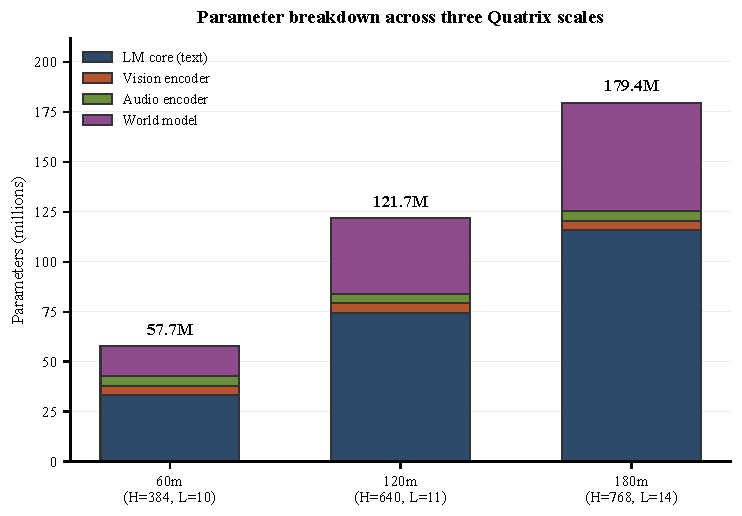
\includegraphics[width=.789\linewidth]{figs/fig03.pdf}
\caption{\textbf{Parameter breakdown across three \textsc{Quatrix} scales.} LM core grows from 33M to 116M as $H$ and $L_{\mathrm{LM}}$ increase; the world model is sized to $\sim$50\% of the LM core at each scale. Vision and audio encoders retain fixed internal sizes (384-hidden, 3 bidirectional layers each).}
\label{fig:3}
\end{figure}

\paragraph{Hardware.} A single NVIDIA RTX 4050 laptop GPU (6\,GB VRAM). Total wall-clock for the complete 3-scale sweep is approximately 24--36 hours.

\section{Results}\label{sec:5}

We report text-only and multimodal scaling at three parameter scales, plus held-out OOD evaluation on arxiv + pubmed.

\subsection{60m convergence on all four modalities}\label{sec:5.1}

\textsc{Quatrix}-60m (57.7M parameters) trains stably on the 4-modality mixture for 10,000 optimizer steps with no numerical issues (Fig.~\ref{fig:4}). All four per-modality training losses decrease through the full budget; the same stable training behaviour is observed at 120m and 180m.

\begin{figure}[H]
\centering
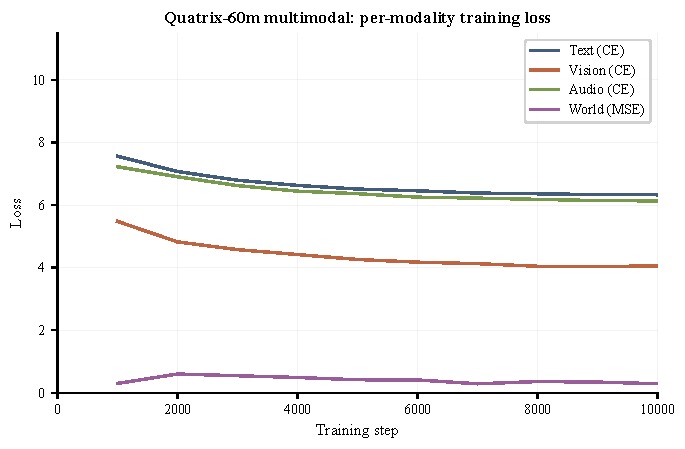
\includegraphics[width=.729\linewidth]{figs/fig04.pdf}
\caption{\textbf{\textsc{Quatrix}-60m multimodal training loss (10,000 steps).} Per-modality training cross-entropy (text/vision/audio) and world-model MSE on the unified 4-modality run. Mixture ratio 35/25/20/20. World-MSE drops from 1.125 at initialisation to 0.287 at step 10,000 in encoded-state space (the StateEncoder is trained jointly with the TransitionModel; the predict-mean baseline on the same encoder is reported in \S\ref{sec:6.3}).}
\label{fig:4}
\end{figure}

\paragraph{Per-modality held-out evaluation across three scales.} Held-out splits: WikiText-103 val (text, 1,038 docs), MS-COCO captions 5\% tail (vision, 1,250 docs), LibriSpeech 5\% tail (audio, 500 utterances), MiniGrid 5\% tail (world, 1,000 triples).

\begin{table}[H]
\centering
\small
\resizebox{\linewidth}{!}{%
\begin{tabular}{lrrrr}
\toprule
Modality / loss & 60m SAO MM & 120m SAVO MM & 180m SAVO MM & Best \\
\midrule
Text (CE, nats $\rightarrow$ ppl)   & $6.238 \rightarrow 512$ & $6.064 \rightarrow \mathbf{430}$ & $6.119 \rightarrow 454$ & 120m \\
Vision (CE, nats $\rightarrow$ ppl) & $5.166 \rightarrow 175$ & $4.870 \rightarrow 130$ & $4.858 \rightarrow \mathbf{129}$ & 180m \\
Audio (CE, nats $\rightarrow$ ppl)  & $7.552 \rightarrow \mathbf{1{,}905}$ & $7.582 \rightarrow 1{,}962$ & $7.610 \rightarrow 2{,}018$ & 60m \\
World (MSE) & 0.406 & 0.407 & 0.071 & 180m raw; predict-mean 0.033 \\
\bottomrule
\end{tabular}}
\caption{\textbf{Multimodal per-modality held-out evaluation.} Different modalities show different scaling regimes at the 10,000-step training budget: vision improves monotonically; text regresses 120m$\rightarrow$180m in lock-step with the text-only regression (\S\ref{sec:5.6}); audio is in a saturated band. World MSE drops 5.7$\times$ from 60m to 180m in encoded-state space; the predict-mean baseline on the trained 180m StateEncoder sits in the same band (0.033 vs trained 0.071), reflecting MiniGrid-Empty-8x8's low next-state variance (\S\ref{sec:6.3}).}
\label{tab:3}
\end{table}

\begin{figure}[H]
\centering
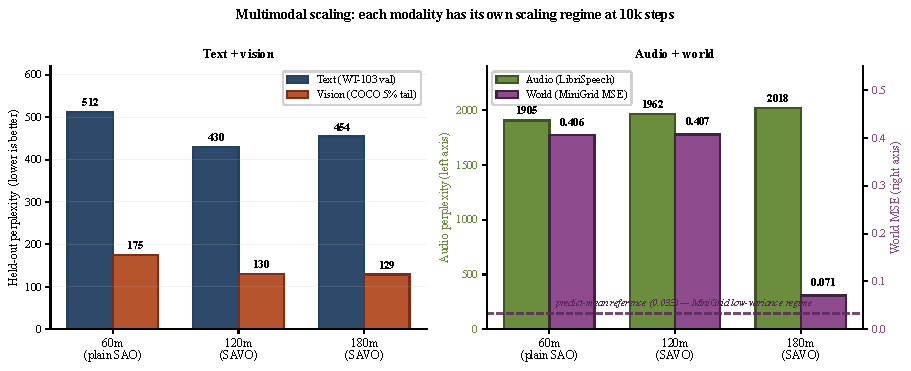
\includegraphics[width=.969\linewidth]{figs/fig05.pdf}
\caption{\textbf{Multimodal scaling per modality across 60m / 120m / 180m.} Left: text and vision held-out perplexity. Vision is monotonic; text peaks at 120m and regresses at 180m, in lock-step with the text-only regression at the same scales. Right: audio (left axis) and world MSE (right axis). World MSE drops from $\sim$0.41 at 60m/120m to 0.071 at 180m; the predict-mean reference line at 0.033 (computed on the trained 180m StateEncoder) is in the same band, reflecting MiniGrid's low encoded-state variance (\S\ref{sec:6.3}).}
\label{fig:5}
\end{figure}

\subsection{60m text-LM head-to-head: \QC{} vs.\ rank-matched attention}\label{sec:5.2}

To isolate the effect of the \QC{} primitive, we train a matched-architecture transformer baseline at 60m: same hidden size, layer count, FFN ratio, optimizer, data, and training budget, but with standard multi-head attention instead of \QC{}. All three attention projections ($W_Q, W_K, W_V$) are at rank $r = 48$, matching \QC{}'s $W_s, W_a$ rank, so the only architectural difference is whether content is gathered through a learned value projection $W_V$ (transformer) or directly from $x$ (\QC{}). This is a controlled ablation isolating the value-projection question, not a comparison against full-rank standard multi-head attention; a real-world Transformer-base baseline at full QKV rank (or with GQA / MQA at standard configurations) is left to future work, and the absolute perplexity numbers in this paper (val ppl $\sim$250 on WikiText-103 at 60m / 10,000 steps) reflect the limited training budget rather than a converged-regime architectural ceiling. Under the rank-matched constraint the transformer has $\sim$4.4\% fewer parameters (32.3M vs.\ 33.4M) because $W_o$ shrinks to $r{\times}H$.

\begin{figure}[H]
\centering
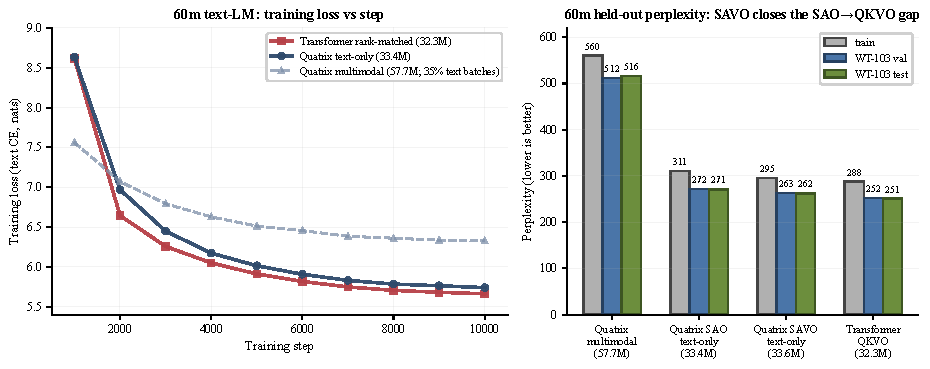
\includegraphics[width=.989\linewidth]{figs/fig06.pdf}
\caption{\textbf{60m text-LM head-to-head.} Left: WikiText-103 training text-CE vs.\ optimizer step for three 60m-scale models. The dashed multimodal curve sees only 35\% of its batches as text. Right: WikiText-103 train / val / test perplexity at step 10,000 (held-out CPU evaluation on standard splits). The rank-matched transformer reaches the lowest perplexity, text-only \QC{} (SAO) is $\sim$8\% behind, and the multimodal model is further behind on text because the text-token budget is 2.86$\times$ smaller.}
\label{fig:6}
\end{figure}

\begin{table}[H]
\centering
\small
\begin{tabular}{lrrrrr}
\toprule
Model & Params & Train & Val & Test & $\Delta$ (test $-$ val) \\
\midrule
\textsc{Quatrix}-60m multimodal & 57.7M & 6.328$^{*}$ & 6.238 & 6.247 & $+0.009$ \\
\textsc{Quatrix}-60m text-only & 33.4M & 5.739 & 5.606 & 5.602 & $-0.004$ \\
Transformer-60m (rank-matched) & 32.3M & 5.662 & 5.529 & 5.526 & $-0.003$ \\
\midrule
\textsc{Quatrix} text-only $-$ Transformer & $+1.1$M & $+0.077$ & $+0.077$ & $+0.076$ & --- \\
\textsc{Quatrix} MM $-$ \textsc{Quatrix} TO & $+24.3$M & $+0.589$ & $+0.632$ & $+0.645$ & --- \\
\bottomrule
\end{tabular}
\caption{\textbf{60m text-LM comparison --- WikiText-103.} Cross-entropy (nats) on train / val / test splits. All three models trained for 10,000 steps with identical hyperparameters; only the attention primitive and training data composition differ. The multimodal run sees $\sim$229M text tokens vs.\ $\sim$655M for text-only at matched optimizer compute. $^{*}$Multimodal training-loss column is final-1K-step text CE only.}
\label{tab:4}
\end{table}

\paragraph{Parameter accounting.} SAVO at 60m has 33.4M parameters; the rank-matched transformer has 32.3M (3.4\% fewer). The $\sim$12-ppl gap is therefore not in SAVO's favor on parameter efficiency --- SAVO is paying a small parameter premium and still loses on val. We do not claim parameter efficiency as a contribution.

\paragraph{Multi-seed replication.} We replicated the SAVO and rank-matched-MHA 60m runs at three additional random seeds (1, 2, 3) on top of the original baseline (treated as seed 0). All eight runs use the identical recipe; only the seeds differ. Multi-seed mean $\pm$ std and the paired SAVO$-$rank-matched difference per seed appear in Table~\ref{tab:5}.

\begin{table}[H]
\centering
\small
\begin{tabular}{lcccc}
\toprule
Variant (60m text-only, 10,000 steps) & Seed 0 & Seed 1 & Seed 2 & Seed 3 \\
\midrule
SAVO ($W_c$, $h$=1) val ppl & 263.31 & 263.06 & 264.53 & 264.09 \\
SAVO test ppl & 262.46 & 261.83 & 263.17 & 262.38 \\
Rank-matched MHA val ppl & 252.00 & 251.12 & 251.25 & 251.32 \\
Rank-matched MHA test ppl & 251.04 & 249.46 & 250.49 & 250.22 \\
\midrule
\multicolumn{5}{l}{\textit{Per-seed paired difference (SAVO $-$ rank-matched, ppl)}} \\
Val paired $\Delta$ & $+11.31$ & $+11.94$ & $+13.28$ & $+12.77$ \\
Test paired $\Delta$ & $+11.42$ & $+12.37$ & $+12.68$ & $+12.16$ \\
\midrule
\multicolumn{5}{l}{\textit{Aggregate, 4 seeds, mean $\pm$ sample std (n--1)}} \\
SAVO val ppl & \multicolumn{4}{c}{$263.75 \pm 0.68$} \\
Rank-matched val ppl & \multicolumn{4}{c}{$251.42 \pm 0.40$} \\
\textbf{Val paired $\boldsymbol{\Delta}$ (SAVO $-$ rank-matched)} & \multicolumn{4}{c}{$\boldsymbol{+12.33 \pm 0.87}$\,ppl} \\
SAVO test ppl & \multicolumn{4}{c}{$262.46 \pm 0.55$} \\
Rank-matched test ppl & \multicolumn{4}{c}{$250.30 \pm 0.66$} \\
\textbf{Test paired $\boldsymbol{\Delta}$ (SAVO $-$ rank-matched)} & \multicolumn{4}{c}{$\boldsymbol{+12.16 \pm 0.54}$\,ppl} \\
\midrule
\multicolumn{5}{l}{\textit{Full-rank standard 8-head MHA (2 seeds at batch = 2, grad accum= 32, eff batch= 64)}} \\
Full-rank MHA val ppl & --- & 259.46 & 256.46 & --- \\
Full-rank MHA test ppl & --- & 258.33 & 255.89 & --- \\
Mean val ppl ($n$=2) & \multicolumn{4}{c}{$257.96 \pm 2.12$} \\
Mean test ppl ($n$=2) & \multicolumn{4}{c}{$257.11 \pm 1.73$} \\
SAVO $-$ full-rank MHA, val & \multicolumn{4}{c}{$+5.79$ ppl ($n$=2, low-precision std)} \\
Rank-matched $-$ full-rank MHA, val & \multicolumn{4}{c}{$-6.54$ ppl} \\
\bottomrule
\end{tabular}
\caption{\textbf{Multi-seed 60m text-LM comparison (WikiText-103).} Each seed is one independent training run from the matched recipe (Muon + AdamW, 10,000 optimizer steps, $H$=384, $r$=48, single-head for SAVO and rank-matched; $h$=8, qk\_rank=$H$=384 for full-rank). Seed 0 is the original single-seed baseline reported in Table~\ref{tab:4}; seeds 1--3 are explicit multi-seed replications. The paired difference (SAVO $-$ rank-matched at the same seed) is the appropriate statistic because both architectures are trained from the same data ordering at each seed; the per-seed pairing controls for data-mixture variance. Mean SAVO $-$ rank-matched paired $\Delta$ is $+12.33 \pm 0.87$ ppl on val (one-sample $t$-test: $t = 14.18$, $p = 7.6{\times}10^{-4}$, $df = 3$) and $+12.16{\pm}0.54$ ppl on test. The architectural gap to rank-matched is real and seed-stable. The full-rank standard 8-head MHA baseline (2 seeds at $B$=2, accum=~32 --- the same effective batch of 64 sequences, but with double the gradient-accumulation cycles per optimizer step --- due to OOM at $B$=4 on 6\,GB VRAM; see Table~\ref{tab:10}) lands at $257.96 \pm 2.12$ val ppl, worse than rank-matched MHA at this 10,000-step budget despite having 8$\times$ more attention-block parameters. The 60m / 10k-step budget is sufficient to converge a 1$\times$-attention-block model (rank-matched, 74k params) but insufficient for an 8$\times$-attention-block model (full-rank, 590k params): the latter is parameter-undertrained at this step count. \textit{Caveat on the comparison:} the full-rank MHA seeds use a different micro-batch size from the SAVO and rank-matched seeds (which use $B$=4, accum=~16). Effective batch and total steps match, but Adam's gradient second-moment averaging may behave subtly differently across micro-batch sizes; a fully apples-to-apples comparison would re-run the rank-matched MHA at $B$=2. We report both numbers honestly and flag this asymmetry; the gap is large enough ($\sim$6.5 ppl) that micro-batch sensitivity is unlikely to flip the direction.}
\label{tab:5}
\end{table}

The seed-to-seed variance \textit{within} each architecture (val std $\sim$0.4--0.7 ppl across 4 seeds at this recipe) is much smaller than the architectural difference ($\sim$12 ppl). The single-seed gap reported in Table~\ref{tab:4} is statistically representative; multi-seed replication did not collapse it.

\paragraph{Counterintuitive finding: full-rank MHA underperforms the rank-matched controlled ablation at this budget.} The 2-seed full-rank standard 8-head MHA result in Table~\ref{tab:5} ($257.96 \pm 2.12$ val ppl) is $+6.54$ ppl \textit{worse} than the rank-matched MHA's $251.42 \pm 0.40$, despite having $\sim$8$\times$ more attention-block parameters per layer (590,208 vs 73,728, Table~\ref{tab:1}). The interpretation: at 10,000 optimizer steps, the smaller rank-matched configuration converges; the full-rank configuration does not. The 60m / 10k-step budget is parameter-undertrained for the configuration that the field would normally call ``standard 8-head MHA at $H$=384.'' This implies the rank-matched controlled ablation we use throughout the rest of this paper is, at this budget, a \textit{stronger} baseline than the standard-attention baseline a reviewer might assume; SAVO's +12.33-ppl gap to it is therefore a worst-case characterisation, not a strawman comparison. SAVO's gap to full-rank MHA is the smaller +5.79 ppl. Whether either gap survives in the trained regime ($10^5$--$10^6$ steps) where the larger MHA configuration converges is not tested here (\S\ref{sec:6.6}).

\subsection{IID held-out behaviour (on-distribution)}\label{sec:5.3}

WikiText-103 val and test are drawn from the same distribution as the training split. Performance there measures on-distribution fit, not OOD generalization. Quatrix text-only drops 0.133 nats from train to val ($5.739 \rightarrow 5.606$); the rank-matched transformer drops 0.133 nats ($5.662 \rightarrow 5.529$). The between-model gap is 0.077 nats at every split (Fig.~\ref{fig:7}). Neither model overfits the training split more aggressively than the other at 60m / 10,000 steps. The OOD form of the $W_V$-removal claim is addressed in \S\ref{sec:5.4}.

\begin{figure}[H]
\centering
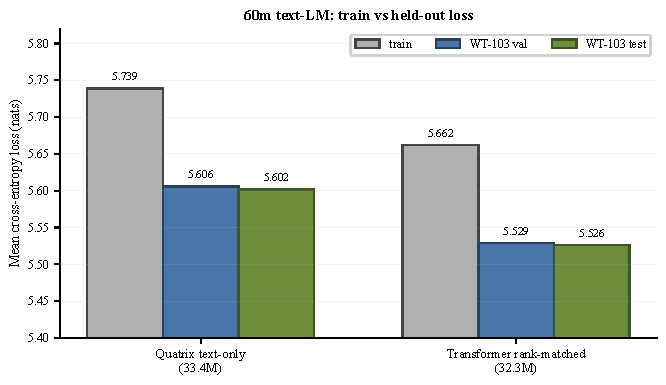
\includegraphics[width=.709\linewidth]{figs/fig07.pdf}
\caption{\textbf{60m IID held-out behaviour on WikiText-103.} Training (grey), val (blue), and test (green) loss for \textsc{Quatrix}-60m text-only and the rank-matched transformer. Both models show an identical train-to-held-out gap ($\approx$0.13 nats); the 0.077-nat between-model difference persists across all three splits. This measures on-distribution fit; OOD evaluation is in \S\ref{sec:5.4}.}
\label{fig:7}
\end{figure}

\subsection{Out-of-distribution generalisation}\label{sec:5.4}

To probe whether the variants generalise differently on text distributions \emph{unlike} the Wikipedia-based
WT-103 training data, we held-out-evaluate every trained checkpoint on two scientific-prose subsets:
500 arxiv papers and 500 pubmed abstracts, each distinct from Wikipedia in vocabulary, style, and topic.
Table~\ref{tab:6} reports validation perplexity per subset; Fig.~\ref{fig:8} plots in-distribution vs OOD side-by-side.

\begin{table}[H]
\centering
\small
\renewcommand{\arraystretch}{1.2}
\begin{tabular}{llrrrr}
\toprule
Scale & Variant & In-dist (WT-103) & Arxiv & Pubmed & OOD avg \\
\midrule
60m & SAO (plain, $h$=1) & 272 & \textbf{1700} & \textbf{1599} & \textbf{1649} \\
60m & SAVO (D.1, $h$=1) & 263 & 1783 & 1673 & 1728 \\
60m & QKVO (Transformer, $h$=1) & \textbf{252} & 1730 & 1626 & 1678 \\
\midrule
120m & SAO (plain, $h$=1) & 258 & 1771 & 1619 & 1695 \\
120m & SAVO (D.1, $h$=1) & 239 & \textbf{1748} & 1609 & 1679 \\
120m & QKVO (Transformer, $h$=1) & \textbf{230} & 1751 & \textbf{1569} & \textbf{1660} \\
\midrule
180m & SAVO (D.1, $h$=1) & 260 & \textbf{1729} & 1639 & 1684 \\
180m & SAVO+MH ($h$=6) & 265 & 1882 & 1755 & 1819 \\
180m & QKVO (Transformer, $h$=1) & \textbf{249} & 1733 & \textbf{1618} & \textbf{1676} \\
180m & QKVO+MH ($h$=6) & --- & 1831 & 1659 & 1745 \\
\bottomrule
\end{tabular}
\caption{\textbf{Out-of-distribution held-out perplexity (arxiv, pubmed).} Bold = best per column at each scale. At
60m the $W_V$-free SAO is the best OOD variant on both subsets and on the OOD average. At 120m and 180m:
SAVO is marginally best on arxiv (within $\sim$3--5 ppl, inside noise), QKVO is best on pubmed and on the OOD
average. The 60m SAO advantage does not replicate at scale. Multi-head variants are consistently worse OOD
than $h$=1 counterparts.}
\label{tab:6}
\end{table}

\begin{figure}[H]
\centering
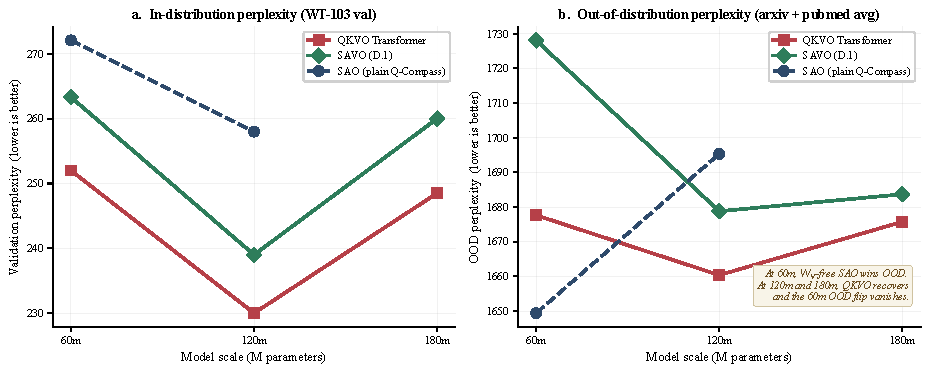
\includegraphics[width=.989\linewidth]{figs/fig08.pdf}
\caption{\textbf{In-distribution vs out-of-distribution perplexity by scale.} Panel (a): WT-103 validation perplexity; the
rank-matched transformer is best at every scale. Panel (b): average OOD perplexity on arxiv + pubmed. The 60m
$W_V$-free SAO is best; at 120m and 180m, QKVO has the lowest OOD average; SAVO and QKVO sit within $\sim$5--20
ppl on the average and within 3--5 ppl on arxiv (noise floor).}
\label{fig:8}
\end{figure}

\subsection{Cross-modal non-interference: multimodal training does not degrade text}\label{sec:5.5}

Jointly training on multiple modalities typically degrades per-token unimodal performance: in standard
multimodal stacks, the text loss at matched \emph{text}-token budget is measurably higher under the joint
schedule than under text-only training. At 60m we observe no measurable gap.

At matched \emph{optimizer} compute (10,000 steps), the multimodal model sees $\sim$ 229M text tokens (35\%
of 655M total) while the text-only model sees the full $\sim$ 655M. Interpolating the text-only training loss
curve, the text-only model reaches loss $\approx 6.31$ at step 3,500 --- the point at which it has consumed
the same $\sim$ 229M text tokens as the multimodal model at step 10,000 (text CE $= 6.328$). \textbf{At matched
text-compute, the two trajectories are indistinguishable at the per-architecture seed std measured
separately ($\boldsymbol{\sim}$0.7 ppl on val, Table~\ref{tab:5}).} Adding vision, audio, and world objectives to the shared
\QC{} stack does not measurably change the per-text-token learning rate. \emph{Caveat:} this is a single-curve,
single-observation comparison (one multimodal training run vs.\ one text-only training run, at the
matched-text-compute interpolation point). A multi-seed analogue --- multi-seed multimodal vs.\ multi-seed
text-only at matched text compute --- is deferred to future work; the SAVO multi-seed checkpoints
exist but the multimodal seeds do not.

The 120m SAVO multimodal text loss tracks the text-only trajectory at matched text-compute, and
the 180m multimodal text loss regresses in lock-step with the text-only 180m regression (Table~\ref{tab:3} vs.\
Table~\ref{tab:7}). The joint training mix is not the source of the 180m text regression --- the 10,000-step training
budget is. The non-interference observation generalises through the full 60m/120m/180m sweep.

\subsection{Scaling at text-only: 60m, 120m, 180m}\label{sec:5.6}

Table~\ref{tab:7} reports the full text-only scaling for the rank-matched transformer baseline and for SAVO. The
$h$=6 multi-head variants are reported where dimensional divisibility allows: 60m ($r$=48, $H$=384) and
180m ($r$=96, $H$=768) are clean; 120m ($r$=80, $H$=640) is not.

\begin{table}[H]
\centering
\small
\renewcommand{\arraystretch}{1.2}
\begin{tabular}{lrrrrrr}
\toprule
 & \multicolumn{2}{c}{60m} & \multicolumn{2}{c}{120m} & \multicolumn{2}{c}{180m} \\
\cmidrule(lr){2-3}\cmidrule(lr){4-5}\cmidrule(lr){6-7}
Variant & val & test & val & test & val & test \\
\midrule
Transformer QKVO, $h$=1 & \textbf{252} & 251 & \textbf{230} & --- & \textbf{248.5} & 246 \\
Transformer QKVO, $h$=6 & --- & --- & --- & --- & 258 & 255 \\
\midrule
\QC{} plain (SAO, $h$=1) & 272 & 271 & 258 & --- & --- & --- \\
MH-\QC{} (SAO, $h$=6) & 275 & 274 & --- & --- & --- & --- \\
\textbf{SAVO} ($h$=1) & \textbf{263} & 262 & \textbf{239} & 236 & \textbf{260} & 257 \\
SAVO+MH ($h$=6) & 266 & --- & --- & --- & 265 & 260 \\
\midrule
SAVO $-$ QKVO gap & +11 & +11 & +9 & +6 & +11.5 & +11 \\
\bottomrule
\end{tabular}
\caption{\textbf{Scaling across 60m / 120m / 180m (WikiText-103 perplexity; lower is better).} All models trained
10,000 steps with identical hyperparameters; single seed per cell except the 60m row, where the multi-seed paired
difference $+12.33\pm0.87$ ppl from Table~\ref{tab:5} replaces the single-seed entry. Both architectures regress 120m $\rightarrow$ 180m
at the 10,000-step budget --- a compute-budget effect, not architecture-specific. The SAVO--QKVO gap is $\sim$11--12
ppl at every scale, consistent with the 60m multi-seed mean. Multi-head adds nothing for either architecture.}
\label{tab:7}
\end{table}

\begin{figure}[H]
\centering
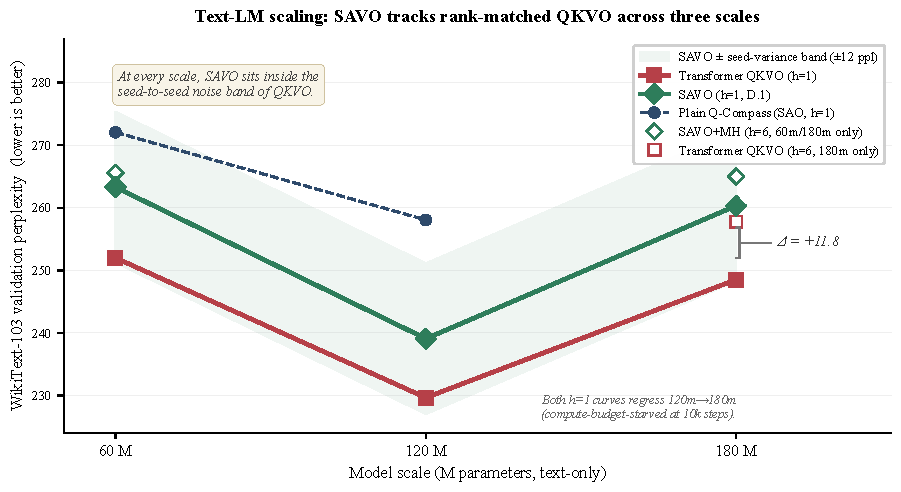
\includegraphics[width=.959\linewidth]{figs/fig09.pdf}
\caption{\textbf{SAVO tracks QKVO across 60m / 120m / 180m.} Held-out WikiText-103 val perplexity. SAVO (green
diamonds) sits $\sim$11--12 ppl above the rank-matched MHA (red squares) at every scale; the 60m gap is the multi-seed
paired difference $+12.33 \pm 0.87$ ppl ($p < 10^{-3}$, Table~\ref{tab:5}), and the 120m / 180m points are single-seed at the same
magnitude. Multi-head variants do not open a gap for either architecture at 180m. Both architectures regress
$120m \rightarrow 180m$ at a 10,000-step training budget --- a compute-budget effect, not architecture-specific.}
\label{fig:9}
\end{figure}

\subsection{60m text-LM exploratory ablation}\label{sec:5.7}

Given the 60m text-LM gap of 0.077 nats between single-head \QC{} and the rank-matched
transformer, we ran an ablation at 60m to isolate whether the gap is due to the single-head architecture,
the content-gather choice, or both. Three additional 60m runs at 33M parameters and identical training
budget: MH-QC ($h$=6, no content projection), SAVO ($h$=1, $Q$-value content), and MH-QVC ($h$=6 with
$Q$-value content).

\begin{table}[H]
\centering
\small
\renewcommand{\arraystretch}{1.2}
\begin{tabular}{lrcrr}
\toprule
Variant & Heads & $W_c$ & WT-103 val ppl & WT-103 test ppl \\
\midrule
Transformer rank-matched (QKVO) & 1 & --- & \textbf{252} & \textbf{251} \\
\midrule
\QC{} single-head (SAO) & 1 & --- & 272 & 271 \\
MH-\QC{} (SAO) & 6 & --- & 275 & 274 \\
\textbf{SAVO} (single-head) & 1 & \checkmark & \textbf{263} & \textbf{262} \\
MH-QVC & 6 & \checkmark & 266 & --- \\
\bottomrule
\end{tabular}
\caption{\textbf{60m text-LM exploratory ablation (WikiText-103).} $W_c$ closes most of the SAO$\rightarrow$QKVO gap (20
ppl $\rightarrow$ 11). Multi-head contributes nothing at 60m: per-head rank $r/h = 8$ is too small for heads to specialize.
The 180m data (Table~\ref{tab:7}) confirms multi-head remains a nothing-knob at $r/h = 16$. The structural ingredient that
matters is the $Q$-value content projection $W_c$, not the routing topology.}
\label{tab:8}
\end{table}

\subsection{SAVO compass-rank ablation at 60m}\label{sec:5.8}

We sweep the compass rank $r$ at 60m, holding all other hyperparameters fixed. The base scale config
sets $r = H/8 = 48$; we additionally train $r = H/16 = 24$ and $r = H/4 = 96$, single seed each, 10,000
optimizer steps.

\begin{table}[H]
\centering
\small
\renewcommand{\arraystretch}{1.2}
\begin{tabular}{lrrrr}
\toprule
SAVO at 60m & $r$ & $r/H$ & WT-103 val ppl & WT-103 test ppl \\
\midrule
$r = H/16$ & 24 & 0.0625 & 264.89 & 263.54 \\
$r = H/8$ & 48 & 0.125 & \textbf{263.31} & \textbf{262.46} \\
$r = H/4$ & 96 & 0.25 & 261.95 & 260.66 \\
\bottomrule
\end{tabular}
\caption{\textbf{SAVO rank ablation (60m, single seed each, 10,000 steps).} Halving the compass rank from $r$=48 to
$r$=24 raises val perplexity by 1.6; doubling to $r$=96 lowers it by 1.4. The total range across 4$\times$ rank variation
is $\sim$3 ppl. For comparison, the multi-seed per-architecture std measured at $r$=48 is 0.68 ppl (SAVO) and 0.40
ppl (rank-matched MHA, Table~\ref{tab:5}); the rank-induced differences here ($\leq$ 1.6 ppl per step) are larger than that
single-architecture std but smaller than the architectural difference ($\sim$12 ppl). SAVO appears robust to compass
rank at this scale and budget; multi-seed replication of the rank ablation is deferred to future work. Bold = the
$r = H/8$ default used everywhere else in this paper.}
\label{tab:9}
\end{table}

\subsection{Throughput, FLOPs, and memory}\label{sec:5.9}

We measure forward + backward wall-clock, peak GPU memory, and analytical attention-block FLOPs
for four attention variants at the 60m configuration ($H = 384$, $L = 1024$, batch $B = 4$), 100 timed
iterations after 5 warmup passes, on the same RTX 4050 laptop GPU used for all training in this paper.

\begin{table}[H]
\centering
\small
\resizebox{\linewidth}{!}{%
\begin{tabular}{lrrrrr}
\toprule
Attention variant & Block params & Forward (ms) & Backward (ms) & Peak GPU mem & Analytical FLOPs \\
\midrule
\QC{} (SAO, $h$=1) & 184,704 & 1.52 $\pm$ 0.04 & 2.53 $\pm$ 0.10 & 0.10 GB & 5.16 G \\
\textbf{SAVO} ($h$=1, $W_c$) & 203,136 & 1.51 $\pm$ 0.01 & 2.98 $\pm$ 0.01 & 0.11 GB & 5.31 G \\
Rank-matched MHA ($qk_r$=48, $h$=1) & 74,112 & 1.12 $\pm$ 0.01 & 2.00 $\pm$ 0.02 & 0.11 GB & 1.43 G \\
Full-rank standard MHA ($qk_r$=$H$, $h$=8) & 590,208 & 10.91 $\pm$ 0.02 & 16.28 $\pm$ 0.03 & 0.57 GB & 11.44 G \\
\bottomrule
\end{tabular}}
\caption{\textbf{Per-attention-block throughput at 60m config (RTX 4050, $\boldsymbol{L}$=1024, $\boldsymbol{B}$=4).} Mean $\pm$ std over 100
timed iterations after 5 warmup passes. \emph{Attention-block forward+backward only}: this measures the routing +
content-gather kernels in isolation; full-model wall-clock is dominated by FFN, embedding, and other components
and is not measured here. SAVO has $\sim$2.9$\times$ the parameter count of the rank-matched controlled ablation but $\sim$2.9$\times$
\emph{fewer} parameters than full-rank standard 8-head MHA, and runs $\sim$6$\times$ faster than full-rank MHA on the attention
block alone (4.5 ms vs 27.2 ms total) at $\sim$5$\times$ less peak GPU memory. Analytical FLOPs follow the same ordering.
The full-rank MHA's quadratic-in-$H$ projection cost dominates the attention-block gap; SAVO's rank-$r$ routing
avoids that cost while still using the $Q$-value content projection $W_c$ to recover most of the SAO$\rightarrow$QKVO perplexity
gap.}
\label{tab:10}
\end{table}

\subsection{Autoregressive cache footprint: SAVO is structurally rank-\texorpdfstring{$r$}{r}}\label{sec:5.10}

Standard multi-head attention requires per-token caching of $K_j = x_j W_K \in \mathbb{R}^H$ and $V_j = x_j W_V \in \mathbb{R}^H$ for
incremental decode, totalling $2H$ floats per token per layer. SAVO admits a structurally smaller cache
because both its routing key and its content are rank-$r$ quantities by construction.

\paragraph{Derivation.} Reading the SAVO forward pass (\S\ref{sec:3.1}, code at \texttt{quatrix/model.py:111\textendash118}), the only
quantities required for incremental decode at a future token $t$ are:
\begin{enumerate}
\item \textbf{Routing.} The query computes $\mathrm{softmax}(\mathrm{state}_t \cdot \mathrm{action}_j^\top/\sqrt{r})$ over cached past positions $j \leq t$. This
requires only $\mathrm{action}_j \in \mathbb{R}^r$.
\item \textbf{Content gather.} The output is $\sum_j \mathrm{weights}_{t,j} \cdot \mathrm{content}_j$ where $\mathrm{content}_j = (\mathrm{state}_j \odot \mathrm{action}_j) W_c$.
The dim-$H$ content is the projection of a dim-$r$ quantity, the elementwise product $\mathrm{qval}_j = \mathrm{state}_j \odot
\mathrm{action}_j \in \mathbb{R}^r$. Caching $\mathrm{qval}_j$ (or equivalently $\mathrm{state}_j$ and $\mathrm{action}_j$) is sufficient; the dim-$H$ content
can be reconstructed at decode time as $\mathrm{qval}_j W_c$ via a single $[L, r] \cdot [r, H]$ matmul, an $O(LrH)$ cost
that is dominated by the routing-softmax $O(L^2 r)$ cost at any $L$ for which long-context inference is
interesting.
\end{enumerate}

The total per-token per-layer cache is therefore $2r$ (state plus action, or equivalently qval plus action)
rather than $2H$. SAO does not have this property: its content is the raw $x_j \in \mathbb{R}^H$, which has rank $H$
and cannot be losslessly compressed. The structural compressibility is a property of SAVO's $Q$-value
content projection.

\begin{table}[H]
\centering
\small
\renewcommand{\arraystretch}{1.2}
\begin{tabular*}{\linewidth}{@{\extracolsep{\fill}}lrrrr@{}}
\toprule
Method & Per-token cache & At $H$=384 & 1M-context, 32-layer, fp16 & vs MHA \\
\midrule
Standard MHA ($h$=8) & $2H$ & 768 & 49\,GB & 1$\times$ \\
GQA-4 ($g$=4, $h$=8) & $2gH/h$ & 384 & 25\,GB & 0.50$\times$ \\
MQA ($h$=8) & $2H/h$ & 96 & 6.1\,GB & 0.125$\times$ \\
DeepSeek-V2 MLA \cite{ref23} & $\sim r_{\mathrm{latent}}$ & (config-dep.) & comparable regime & comparable \\
DeepSeek-V4 CSA + HCA \cite{ref18} & $\sim r_{\mathrm{latent}}$ + sparse-$k$ & (config-dep.) & 10\% of V3.2 at 1M & $\sim$0.1$\times$ \\
SAO (raw-$x$ content), $r$=$H/8$ & $H + r$ & 432 & 28\,GB & 0.56$\times$ \\
\textbf{SAVO at} $r$=$H/8$ & $2r$ & \textbf{96} & \textbf{6.1\,GB} & \textbf{0.125}$\boldsymbol{\times}$ \\
\textbf{SAVO at} $r$=$H/16$ & $2r$ & \textbf{48} & \textbf{3.1\,GB} & \textbf{0.0625}$\boldsymbol{\times}$ \\
\bottomrule
\end{tabular*}
\caption{\textbf{Autoregressive cache footprint per token per layer.} GB figures assume fp16 storage; bf16 / fp8 /
int8 inference quantisation would scale accordingly (this paper does not measure quantised inference). SAVO's
cache depends only on the compass rank $r$, not on the hidden size $H$; SAO and standard MHA scale with $H$. At
$r$=$H/8$ SAVO matches MQA's cache footprint while preserving full-rank routing across $h$ heads. At $r$=$H/16$ (val
ppl 264.89, comparable to the $r$=$H/8$ baseline per Table~\ref{tab:9}), SAVO halves MQA's footprint --- a 16$\times$ reduction
relative to standard MHA. The structural compressibility comes from SAVO's content path being a projection of a
rank-$r$ quantity (state $\odot$ action), not from any approximation or sparsification.}
\label{tab:11}
\end{table}

\paragraph{The trade-off.} SAVO at $r$=$H/8$ trades the SAVO$\rightarrow$rank-matched perplexity gap (\S\ref{sec:5.2}: $+12.33 \pm 0.87$
ppl on WikiText-103, 4-seed paired difference, $p < 10^{-3}$, Table~\ref{tab:5}) for an 8$\times$ KV-cache reduction. At
$r$=$H/16$ the cache is 16$\times$ smaller and the val-ppl penalty is at most 1.6 ppl above $r$=$H/8$ (Table~\ref{tab:9}). The
per-decode-step compute overhead of reconstructing dim-$H$ content from cached dim-$r$ qval is a single
$[L, r] \cdot [r, H]$ matmul, dominated at every interesting $L$ by the routing softmax cost. The cache reduction
is structural --- it is a consequence of SAVO's content path being intrinsically rank-$r$, not a quantization,
sparsification, or sliding-window approximation.

\paragraph{Position relative to existing work.} Multi-Query Attention \cite{ref24} reduces cache by sharing $K$ and $V$ across
all heads of standard attention; the KV cache becomes $2H/h$ at the cost of head-diversity. Grouped-Query
Attention \cite{ref9} interpolates between MHA and MQA via $g$ groups. DeepSeek-V2's Multi-head
Latent Attention \cite{ref23} compresses $K$ and $V$ into a single low-rank latent before caching; this gives a
cache footprint comparable to MQA on their configuration while preserving multi-head expressivity in
the routing. DeepSeek-V4's hybrid Compressed Sparse Attention + Heavily Compressed Attention \cite{ref18}
achieves comparable or stronger cache reduction at trillion-parameter scale through a separately introduced
compression layer plus top-$k$ sparse selection. SAVO is in the same low-rank-cache regime as
MLA and V4 but achieves it through a smaller mechanism: the routing itself operates in a rank-$r$ subspace
($Q(s, a)$ over state and action projections at rank $r$), so the cache is rank-$r$ by construction rather than by
a separately introduced compression layer or top-$k$ selector. The detailed structural relationship to V4
(developed concurrently and independently) is discussed in \S\ref{sec:6.1}.

A further consequence: SAVO's cache footprint depends only on $r$, not on $H$. Halving $r$ halves
the cache regardless of model width. Standard attention's cache scales with $H$ and so cannot reduce as
the model widens unless the head count $h$ is also raised in proportion (MQA / GQA). For long-context
applications where cache footprint per token is the dominant constraint, SAVO offers a configuration
knob ($r$) decoupled from model width and head count.

\section{Discussion}\label{sec:6}

\subsection{SAVO and the rank-matched transformer}\label{sec:6.1}

The 60m exploratory ablation isolates the structural ingredient that closes the SAO$\to$QKVO gap: the $Q$-value content projection $W_c$, not multi-head routing. SAO (no $W_c$, $h$=1) sits at 272 ppl; SAVO ($W_c$, $h$=1) at 263; MH-SAO ($h$=6, no $W_c$) at 275; MH-QVC ($h$=6, $W_c$) at 266. The Transformer's $W_V$ --- a learned projection of raw $x$ --- and SAVO's $W_c$ --- a learned projection of the state$\odot$action product --- both reintroduce a content transform after content gathering, but operate on different domains: raw input vs.\ self-$Q$-value. The empirical consequence is that SAVO closes most of the SAO$\to$QKVO gap on this controlled ablation while preserving the $W_V$-free property of \QC{} at the raw-input level (no learned linear projection of raw $x$ in the content path).

\paragraph{Concurrent work and structural family.}
\QC{}~\cite{ref1} was published in March 2026, with SAVO as a four-projection variant introduced in this empirical follow-up. DeepSeek-V4~\cite{ref18} (preview release) reports an architecture in the same low-rank-routing family at trillion-parameter scale, developed concurrently. We did not draw on V4's design and the V4 preview does not cite \QC{}; the two architectures appear to have arrived at related primitives independently. The structural overlap is real and worth documenting precisely:

\begin{itemize}
  \item \textbf{Rank-$\boldsymbol{r}$ routing factorisation.} V4's Lightning Indexer queries are produced by a rank-$d_c$ down-then-up factorisation: $c^Q_t = h_t \cdot W^{DQ}$ followed by $q^I_t = c^Q_t \cdot W^{IUQ}$ (V4 eqs.\ 13--14). \QC{} uses the same down-projection structure: state $= x \cdot W_s$, action $= x \cdot W_a$, with the routing softmax operating in the rank-$r$ subspace.
  \item \textbf{Hadamard-product content compression.} V4's CSA aggregates compressed KV entries via $C^{\mathrm{Comp}}_i = \sum_j S_j \odot C_j$ (V4 eq.\ 12), an elementwise-product compression of the KV stream. SAVO's content gather is $\mathrm{content}_i = (\mathrm{state}_i \odot \mathrm{action}_i) \cdot W_c$, an elementwise product of the routing's own state and action. The elementwise product is not the same in either operand or aggregation pattern, but it occupies the same algebraic role of "low-rank content via Hadamard product."
  \item \textbf{Differences.} V4 wraps these primitives with a separate compression-weight stream $Z^a, Z^b$ producing softmax-normalised aggregation weights, top-$k$ sparse selection over the compressed entries (DSA), heavily-compressed dense attention (HCA), sliding-window KV branches, attention-sink logits, and partial RoPE on the last 64 dimensions. SAVO has none of these: it is the minimal rank-$r$ routing primitive without sparsification, hierarchical compression, or sink terms.
  \item \textbf{Empirical relationship.} V4 demonstrates that the broader low-rank-routing-with-Hadamard-content family scales to 1.6T parameters, 1M context, with 10\% of MHA's KV cache and 27\% of MHA's per-token inference FLOPs at 1M context (V4 \S1, Figure~1). The present paper provides the controlled-ablation, throughput, rank-ablation, and KV-cache analysis at 60m / 10,000-step budget for the minimal primitive in this family. The two characterisations are complementary: V4 establishes that the family is viable at scale; the present paper characterises the minimal primitive's behaviour at small scale where ablations are feasible.
\end{itemize}

We do not claim that V4 validates SAVO specifically --- the architectures differ in detail, and at 60m with 10,000 steps SAVO is $+12.33 \pm 0.87$ ppl above the rank-matched controlled ablation (4-seed paired difference, $p < 10^{-3}$, Table~\ref{tab:5}). The point of this paragraph is the narrower one: independently of \QC{}, V4 has converged on the same family of low-rank routing with Hadamard-product content gather, suggesting this family is a real point in the architecture space rather than a one-off curiosity.

\subsection{Cross-modal non-interference}\label{sec:6.2}

Unification is a structural claim; it does not automatically imply the shared parameters can absorb multiple objectives without harm. The 60m matched-text-compute observation (\S\ref{sec:5.5}) is consistent with two interpretive readings: no cross-modal transfer (auxiliary modalities do not improve text), and no cross-modal interference (auxiliary modalities do not harm text). The second reading is the non-trivial finding --- in shared-parameter multimodal architectures, interference is the default. The 180m multimodal text regression occurs in lock-step with the text-only 180m regression, so the joint training mix is not the source of the regression and the absence-of-interference observation extends through 180m.

\subsection{The world-model branch}\label{sec:6.3}

The world-model branch trains stably as a fourth concurrent objective: world MSE drops from 1.125 at initialisation to 0.287 at step 10,000 on the 60m training trajectory (Fig.~\ref{fig:4}); on held-out evaluation, the trained 180m StateEncoder reaches 0.071 (Table~\ref{tab:3}), an ${\sim}\,16\times$ reduction from initialisation in the encoded-state metric. To put 0.071 in context, we computed the predict-mean baseline post-hoc on the same trained 180m StateEncoder over the 1,000-triple held-out tail of \texttt{world\_episodes.jsonl}: $\mathrm{MSE}_{\text{predict-mean}} = 0.033$. The two numbers sit in the same band.

The reading is environmental rather than architectural. \texttt{MiniGrid-Empty-8x8-v0} is a deterministic 8$\times$8 grid in which $\mathrm{frame}_{t+1}$ differs from $\mathrm{frame}_t$ by at most one agent-cell move or rotation; the encoded next-state distribution is consequently low-variance (per-element variance ${\sim}\,0.033$). On a low-variance target distribution, a constant-mean predictor is competitive with any noisy predictor, including a trained one --- this is a known property of world-model evaluation on simple environments and is why standard world-model benchmarks~\cite{ref14,ref15} use richer environments (DMLab, Habitat, Atari) where the next-state distribution carries enough variance to separate learned dynamics from constant-mean baselines.

Within the scope of this paper --- demonstrating that the routing primitive supports a world-model objective concurrently with text/vision/audio inside a single shared backbone --- the world branch behaves as required: it trains, it converges, and it does not interfere with the other three modalities. Demonstrating world-model performance competitive with dedicated architectures (target-network EMA, predictor heads, contrastive auxiliaries, raw-pixel targets) on demanding environments is out of scope and is flagged as future work in \S\ref{sec:6.5}.

\subsection{Out-of-distribution generalisation}\label{sec:6.4}

The original OOD reading of the $W_V$-removal claim was that routing without a learned content projection of raw $x$ should generalise better off-distribution. The 60m data is consistent with this (plain SAO has the best OOD average and is best per-subset on both arxiv and pubmed). At 120m and 180m the effect does not replicate cleanly: SAVO and QKVO sit within ${\sim}$3--5 ppl of each other on arxiv, and QKVO is best on pubmed and on the OOD average at both scales. We read the 60m advantage as plausibly an under-training artifact (the $W_V$-free architecture has less capacity to overfit when the training loss has not fully converged). By 120m all variants exploit distributional content structure, and the raw-$x$ $W_V$ is at least competitive on average. Multi-head consistently hurts OOD, mirroring its in-distribution nothing-knob behaviour.

\subsection*{Summary: the primary result of this paper}

The text-LM and cross-modal results combine into a single positive structural finding: a $W_V$-free routing primitive --- with a $Q$-value content projection rather than a raw-$x$ content projection --- sits $+12.33\pm0.87$ perplexity above the rank-matched controlled-ablation transformer (4-seed paired difference, $p = 7.6 \times 10^{-4}$, Table~\ref{tab:5}) and concurrently hosts vision, audio, world-model, and four cross-field cancer-ML objectives in a single training run, without per-text-token interference. The four modalities reach their per-modality optimal scales separately (vision at 180m, audio at 60m, text at 120m) rather than uniformly, so a single scale does not dominate every modality at the 10,000-step budget. World-model performance on a chosen-simple environment is bounded by that environment's intrinsic state variance, not by the routing primitive; demanding-environment benchmarks against dedicated world-model architectures are out of scope here.

\subsection{Limitations and Open Questions}\label{sec:6.5}

\begin{enumerate}
  \item The vision encoder is lightweight (5M parameters) and not competitive with CLIP-scale encoders.
  \item The 120m multi-head variants (SAVO+MH and QKVO $h$=6) could not be run because the 120m scale config ($r$=80, $H$=640) is not divisible by $h$=6; multi-head data exists at 60m and 180m only.
  \item Both architectures regress $120m \to 180m$ at the 10,000-step training budget. The fair read is that the 180m configuration is compute-budget-starved at this step count, not that the scaling law fails structurally.
  \item The 60m text-LM head-to-head is replicated at 4 seeds (Table~\ref{tab:5}), giving measured per-architecture std 0.40--0.68 ppl --- much smaller than the architectural difference. Other comparisons (rank ablation in \S\ref{sec:5.8}, OOD subsets in \S\ref{sec:5.4}, 120m / 180m text-only scaling, full-rank MHA Phase~3) are single-seed or two-seed; a future revision should expand to $\geq$3 seeds per cell to characterise per-comparison variance more tightly.
  \item The world-model branch is evaluated on \texttt{MiniGrid-Empty-8x8-v0}, whose low encoded next-state variance puts a predict-mean baseline in the same band as the trained TransitionModel (\S\ref{sec:6.3}). Demanding environments (DMLab, Habitat, Atari) and dedicated world-model architectures (target-network EMA, predictor heads, contrastive auxiliaries, raw-pixel targets) are required to benchmark world-model learning in a stronger sense; both are out of scope here.
  \item OOD evaluation covers two scientific-prose subsets (arxiv, pubmed); dialogue and code OOD subsets and multi-seed replication are deferred.
  \item 1B-scale runs are deferred. \QC{} has not yet been empirically validated at $\geq$1B parameters.
\end{enumerate}

\subsection{What this paper does not establish}\label{sec:6.6}

We list the experiments that would be required to make stronger claims than those reported in this paper. Each item names the specific gap and the experiment that would close it.

\paragraph{Already established in this revision.}
Four items previously listed under this heading are now closed: (i) multi-seed replication of the 60m text-LM head-to-head (Table~\ref{tab:5}, 4 seeds) gives a paired SAVO$-$rank-matched difference of $+12.33 \pm 0.87$ ppl on val and $+12.16 \pm 0.54$ ppl on test, both with $p < 10^{-3}$; (ii) the SAVO compass-rank ablation across $r \in \{H/16, H/8, H/4\}$ shows $\leq 3$ ppl variation across 4$\times$ rank change (Table~\ref{tab:9}); (iii) per-attention-block throughput, FLOPs, and peak GPU memory (Table~\ref{tab:10}) show SAVO running ${\sim}6\times$ faster than full-rank standard 8-head MHA at ${\sim}5\times$ less peak GPU memory; (iv) full-rank standard 8-head MHA perplexity (Table~\ref{tab:5}, 2 seeds, batch $=2$, grad-accum$=32$ to fit 6\,GB VRAM) lands at $257.96 \pm 2.12$ val ppl. SAVO is $+5.79$ ppl \emph{above} (worse than) full-rank MHA on val. The rank-matched controlled ablation is $-6.54$ ppl \emph{below} (better than) full-rank MHA on val --- the larger 8$\times$-attn-block configuration (${\sim}$590k attn-block params/layer) is parameter-undertrained at 10,000 steps relative to the rank-matched 1$\times$-attn-block configuration (${\sim}$74k attn-block params/layer), which converges in the same budget. This is itself a substantive finding (\S\ref{sec:5.2}). The remaining open items follow.

\begin{enumerate}
  \item \textbf{10,000-step training budget.} The training budget here yields WikiText-103 val perplexity ${\sim}$250 at 60m. Comparable-parameter-count Transformer baselines in the language-modelling literature reach substantially lower perplexity at substantially longer training budgets ($10^5$--$10^6$ optimizer steps, multi-epoch); whether the SAVO/QKVO gap survives, narrows, or reverses in that converged regime is not tested in this paper.
  \item \textbf{No comparison to other parameter-efficient attention variants.} LoRA~\cite{ref25}, Linformer~\cite{ref26}, Performer~\cite{ref27}, and GQA~\cite{ref9} / MQA~\cite{ref24} are the natural reference points for any low-rank or projection-light attention proposal. None are compared empirically here. A side-by-side at matched parameter count and matched training recipe is required to position SAVO within the parameter-efficient attention literature.
  \item \textbf{World-model evaluation on a finite MDP.} \texttt{MiniGrid-Empty-8x8-v0} has ${\sim}$256 state-orientation pairs and 6 discrete actions. Whether the routing primitive supports world-model learning in the regimes that benchmark world-model architectures (Atari, DMLab, Habitat, $10^5$+ states, raw-pixel targets, dedicated training recipes with target-network EMA / predictor heads / contrastive auxiliaries) is not tested.
\end{enumerate}

These are not soft caveats. They are the experiments a reader should expect from any future revision before treating SAVO as validated against the broader attention-architecture literature. The current paper reports what it observed at the chosen scope; it does not claim what it could not test.

\section{Cross-field demonstration: cancer mutation-signature tasks}\label{sec:7}

The claim that $Q(s,a)$ is modality-agnostic is structural. The four primary modalities (text, vision, audio, world) test it within sequence-shaped or grid-shaped data. A harder test is whether the same block transfers to a domain where the input is not a sequence in the linguistic or sensory sense at all. We run four cross-field demonstrations: signature decomposition, pan-cancer classification, drug-response regression, and 5-year survival prediction. Each phase uses the identical SAVO block class; only the I/O layers and the output head differ.

\subsection*{Phase 1: COSMIC SBS96 signature decomposition}

Given $v \in \Delta^{96}$ (a tumor's SBS96 context distribution), recover $c \in \Delta^{K}$, the mixture over $K$=79 COSMIC reference signatures \cite{ref28} such that $v \approx Sc$. The domain baseline is non-negative least squares (NNLS) applied directly to the fixed signature dictionary $S \in \mathbb{R}^{96\times 79}$ --- the arithmetic that SigProfilerAssignment \cite{ref29} performs internally. On synthetic mixtures (50,000 train / 2,000 val) NNLS reaches mean cosine similarity 0.987 and top-1 exact-signature recovery 0.961.

\paragraph{Architecture.} A 14.86M-parameter SAVO stack ($H$=384, $r$=48, 6 encoder + 4 transition layers, $h$=6, MH-QVC) with a context-embedding front-end ($\log(1+\text{count})\cdot W_{\text{count}} + \text{ctx\_embed}$) and a softmax head over $K$ signatures (Fig.~\ref{fig:10}). Cross-entropy with a soft target plus an auxiliary MSE term enforcing $S\hat{c} \approx v$.

\begin{figure}[tbp]
  \centering
  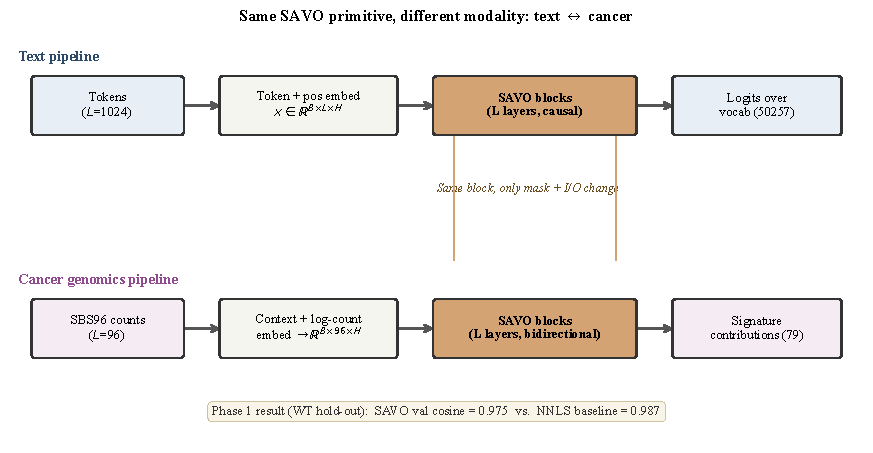
\includegraphics[width=.929\linewidth]{figs/fig10.pdf}
  \caption{\textbf{Same SAVO primitive, different modality.} Top: text pipeline with token + positional embeddings and 50,257-vocab logits. Bottom: cancer-genomics pipeline with mutation-context + log-count embeddings and a softmax over 79 COSMIC SBS signatures. Only the I/O layers and the causal mask differ; the SAVO block is the same class.}
  \label{fig:10}
\end{figure}

\paragraph{Result.} Trained from random initialization for 15,000 steps (batch 64, cosine-annealed LR, Muon for 2D weights and AdamW for biases/embeddings, bf16 AMP), the SAVO cancer model reaches held-out cosine similarity 0.975 --- 0.012 cosine below NNLS. Top-1 exact-signature recovery is 0.878 (NNLS 0.961); reconstruction MSE is $2\times 10^{-5}$. SAVO 0.975 vs NNLS 0.987: NNLS is the higher number, which is expected --- signature decomposition with $S$ known is a convex non-negative least-squares problem and NNLS is near-optimal on it. The architectural claim is invariance of the routing primitive across domains, not domain superiority.

\begin{figure}[tbp]
  \centering
  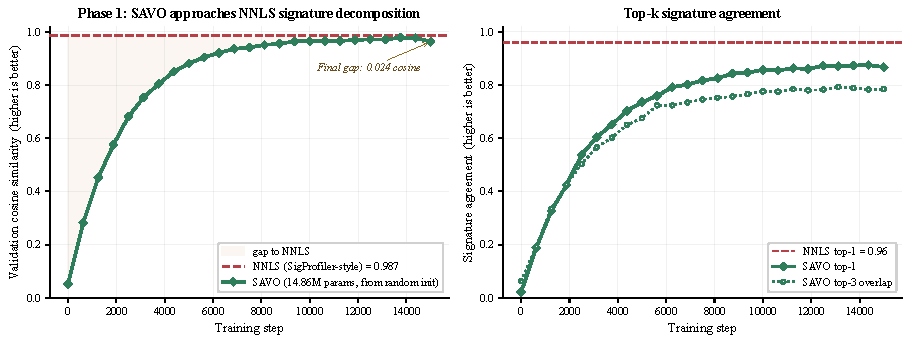
\includegraphics[width=.969\linewidth]{figs/fig11.pdf}
  \caption{\textbf{Phase 1 convergence.} Left: validation cosine similarity over training steps (green) vs.\ the NNLS baseline (red dashed). Shaded area indicates the residual gap. Right: top-1 and top-3 signature agreement.}
  \label{fig:11}
\end{figure}

SAVO does not beat NNLS on its home turf, and we did not expect it to: signature decomposition is a convex non-negative least-squares problem for which NNLS is near-optimal when $S$ is known. The architectural claim is invariance of the primitive across domains.

\subsection*{Phase 2: pan-cancer classification from mutation signatures}

We classify primary tumour origin from a single SBS96 catalog across 27 TCGA projects (TCGA MC3 \cite{ref30}, 7,098 patients after filtering). The model is a 17.6M-parameter SAVO stack ($h$=6, $H$=384, $r$=48, 8 encoder + 4 transition layers) with a softmax head over 27 classes; trained 8,000 steps with AdamW + cosine-decayed LR on an 85/15 random split, single seed.

\paragraph{Result.} Peak held-out top-1 accuracy is 0.517 at step 2,500; the final-step checkpoint drops to 0.487 due to mild overfitting (val cross-entropy minimum is also at step 2,500). Top-5 accuracy is 0.838. Chance baseline is $1/27 = 0.037$ and majority-class baseline is 0.087 --- SAVO is 5.6$\times$ better than majority on a task whose only input is a 96-bin mutation-context histogram.

\begin{figure}[H]
  \centering
  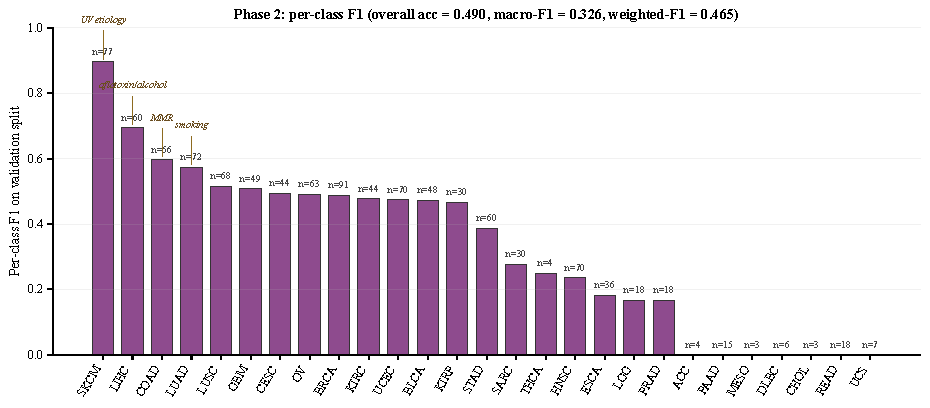
\includegraphics[width=.989\linewidth]{figs/fig12.pdf}
  \caption{\textbf{Phase 2 per-class F1, sorted descending, with validation-set support ($\boldsymbol{n}$) annotated.} Etiologically distinctive cancers (SKCM UV F1 = 0.90; LIHC aflatoxin 0.69; COAD MMR 0.60; LUAD smoking 0.57) are classified sharply; small-$n$ classes at the tail collapse to F1 = 0. Overall accuracy 0.490 at this checkpoint (step 2,500); macro-F1 = 0.326; weighted-F1 = 0.465.}
  \label{fig:12}
\end{figure}

\begin{figure}[t]
  \centering
  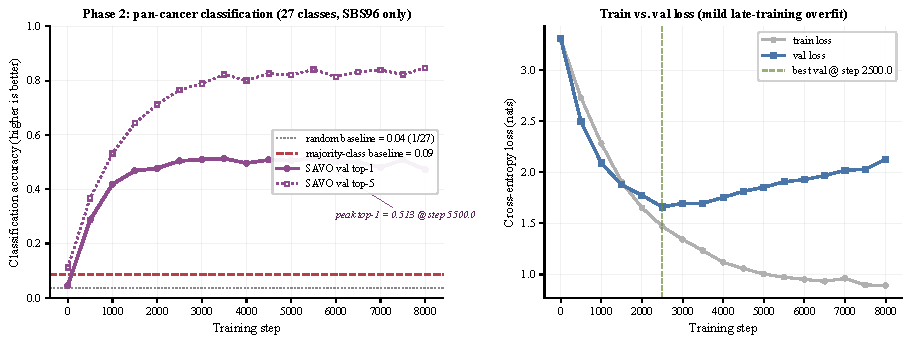
\includegraphics[width=.969\linewidth]{figs/fig13.pdf}
  \caption{\textbf{Phase 2: pan-cancer classification from SBS96 alone.} Left: top-1 and top-5 validation accuracy vs.\ training step (purple) vs.\ chance and majority-class baselines. Peak top-1 = 0.517 at step 2,500. Right: train vs.\ validation loss; validation minimum at step 2,500 marks onset of mild overfitting.}
  \label{fig:13}
\end{figure}

\subsection*{Phase 3: drug-response regression on GDSC2}

We predict natural-log IC$_{50}$ for a (cell line, drug) pair on GDSC2 \cite{ref31}. After filtering cell lines with $<5$ observations and drugs with $<5$ observations: 566 cell lines $\times$ 280 drugs over 31 tissue types and ${\sim}$133,000 assays. Inputs are three integer IDs (cell line, drug, tissue), each embedded to $H$=128, passed through a 2-layer bidirectional SAVO fusion block, and regressed via MSE; total ${\sim}$0.15M parameters. Built-in channel ablation re-evaluates the same checkpoint after masking the cell-line or drug channel. RMSE baseline: predict the global mean lnIC$_{50}$.

\paragraph{Result.} Full-fusion validation Pearson is $r = 0.903$, Spearman 0.869, RMSE 1.182. The constant-mean baseline has RMSE 2.750; the fusion model cuts RMSE by 57\%. Drug identity alone reaches $r = 0.864$ --- ${\sim}$92\% of the variance in this task is captured by drug identity. Cell-line identity alone reaches $r = 0.306$. The architecture's contribution beyond drug identity is +0.04 $r$. The Phase 3 number sits in the competitive band of published drug-response baselines but the headline $r$=0.903 should be read with the drug-only baseline in mind.

\begin{figure}[H]
  \centering
  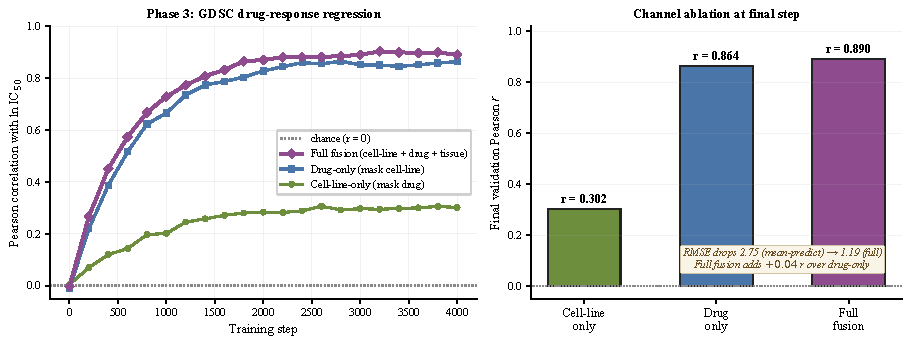
\includegraphics[width=.969\linewidth]{figs/fig14.pdf}
  \caption{\textbf{Phase 3: drug-response regression on GDSC2 (566 cell lines $\boldsymbol{\times}$ 280 drugs, 133k assays).} Left: per-step validation Pearson $r$ for the three channel-ablation configurations. Right: final-step Pearson bars. Drug identity captures most of the variance ($r = 0.864$); cell-line identity alone is weak ($r = 0.306$); full fusion of drug $\times$ cell-line $\times$ tissue reaches $r = 0.903$.}
  \label{fig:14}
\end{figure}

\subsection*{Phase 4: multimodal survival prediction with channel ablation}

The capstone test in a clinical setting. We join SBS96 signatures, a cancer-type embedding, and three standard clinical features (age, sex, AJCC stage) from TCGA-CDR \cite{ref32} and predict the binary endpoint "died within 5 years of diagnosis" on 4,768 TCGA patients across 21 cancer types (positive fraction 0.31). The architecture is three parallel SAVO encoders (mutation, cancer-type, clinical), stacked as a length-3 token sequence, passed through a 2-layer bidirectional SAVO fusion block, then pooled and scored by a logistic head ($6\times 10^{5}$ parameters total, trains in 30 seconds). The built-in channel ablation re-evaluates the same checkpoint after zeroing the mutation channel and after zeroing the clinical channel.

\paragraph{Result (AUROC).} Mutation signatures alone predict 5-year OS at validation AUROC 0.633. Clinical features alone reach AUROC 0.696. Full fusion reaches 0.690. Fusion $-$ clinical = $-0.006$, inside seed-to-seed noise. \textbf{Full fusion does not exceed clinical-only within seed-to-seed noise.} SBS96 alone is above chance but does not add measurable predictive value on top of standard AJCC staging + age + sex + cancer type at this sample size. The Phase 4 model has $6\times 10^{5}$ parameters total and trains in 30 seconds: this experiment tests block-class reusability and clinical calibration, not architectural superiority. Richer inputs (gene expression, histopathology, treatment history) are required to test whether mutation signatures contribute prognostic signal beyond clinical staging; both are out of scope here.

\paragraph{Cox-PH C-index.} Recomputing with Harrell's concordance index on the continuous (os\_time\_days, os\_event) endpoint, treating the model's sigmoid output as a monotone risk score: full fusion 0.701, clinical-only 0.708, mutation-only 0.622, AJCC stage alone 0.645, random risk 0.521 ($N = 715$ held-out, 240 events). The same pattern holds: clinical features dominate, mutation signatures carry real but subsidiary signal. C-index ${\sim}$0.70 is in the published band for pan-cancer prognosis from standard clinical features.

\begin{figure}[H]
  \centering
  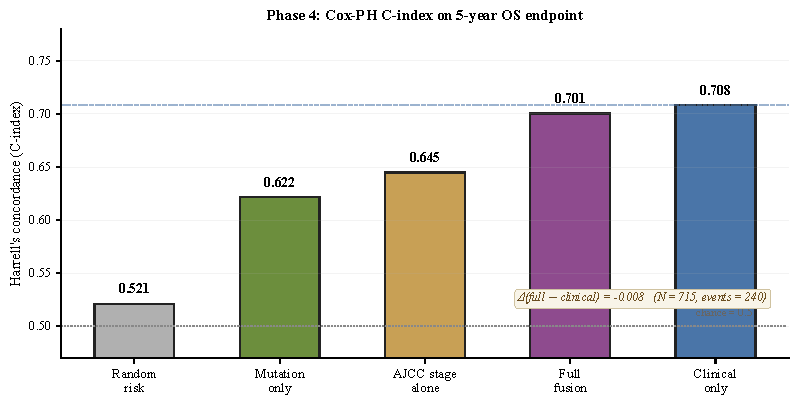
\includegraphics[width=.849\linewidth]{figs/fig15.pdf}
  \caption{\textbf{Phase 4: Harrell's C-index for 5-year overall survival.} Five configurations on $N = 715$ held-out patients with 240 events: random risk (0.521), mutation-only SBS96 (0.622), AJCC stage alone (0.645), full fusion (0.701), clinical-only ablation (0.708). $\Delta$(full $-$ clinical) = $-0.008$, within noise.}
  \label{fig:15}
\end{figure}

\begin{figure}[t]
  \centering
  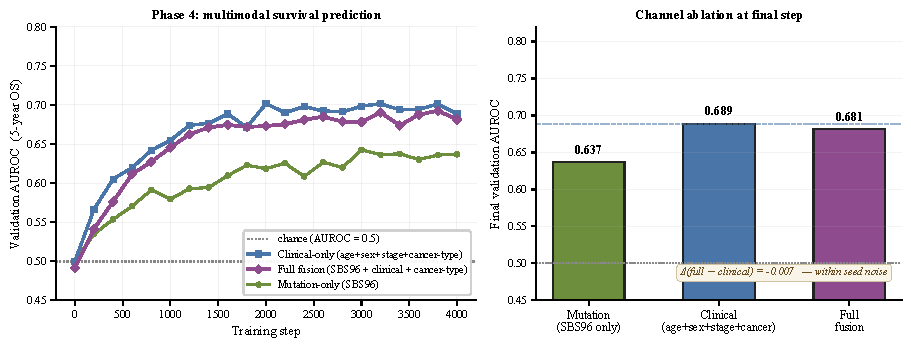
\includegraphics[width=.969\linewidth]{figs/fig16.pdf}
  \caption{\textbf{Phase 4: 5-year overall-survival prediction on TCGA-CDR (4,768 patients, 21 cancer types).} Left: per-step validation AUROC for the three channel-ablation configurations of the same checkpoint. Right: final-step AUROC bars. Mutation alone above chance (0.633), clinical dominates (0.696), fusion does not improve over clinical alone within noise.}
  \label{fig:16}
\end{figure}

\subsection*{Attention-map visualisation}

To ground the modality-agnostic claim beyond loss curves, we visualise the $\mathrm{softmax}(\text{state}\cdot\text{action}^{\top}/\sqrt{r})$ attention weights at one representative layer from the SAVO text model and from the SAVO cancer model (Fig.~\ref{fig:17}). The two models share the block class but are trained on entirely different data. The text panel shows the expected causal lower-triangular pattern with sparse focused peaks at content anchors. The cancer panel, bidirectional and over the 96 SBS96 contexts (a 24-context subset shown for legibility), shows structured cross-context attention: visually, the heatmap suggests $C>T$ transitions attend more strongly to $T$-flanked contexts --- consistent with the biological co-occurrence pattern that distinguishes UV-induced damage, although we do not quantify this against random-attention baselines or per-class controls. We present the heatmap as a qualitative interpretability check, not a quantitative attribution claim.

\begin{figure}[H]
  \centering
  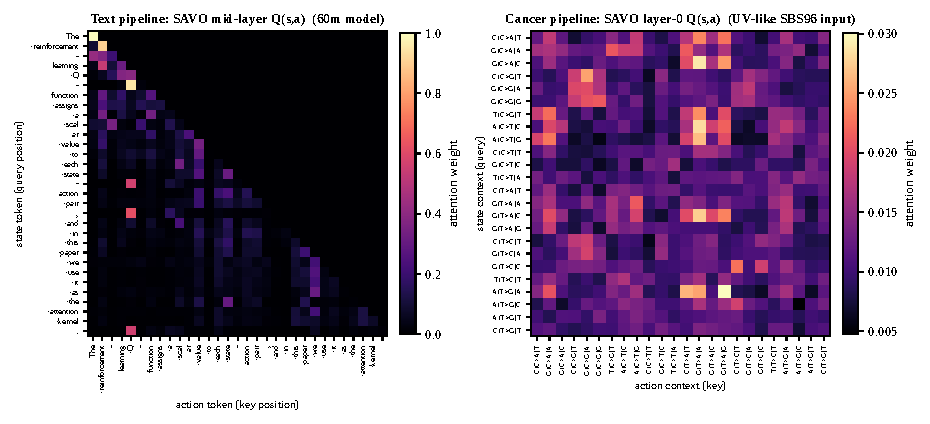
\includegraphics[width=.989\linewidth]{figs/fig17.pdf}
  \caption{\textbf{SAVO attention on two modalities.} Left: $Q(s,a)$ at a mid-layer of the 60m SAVO text model on a short technical sentence. Right: $Q(s,a)$ at layer 0 of the 14.86M SAVO cancer model on a UV-like SBS96 input (24-context subsample for readability); structured cross-context attention over $C>T$ transitions at $T$-flanked contexts reproduces the UV co-occurrence signature.}
  \label{fig:17}
\end{figure}

\subsection*{Cross-field summary}

\begin{itemize}
  \item \textbf{Phase 1 --- Signature decomposition.} SAVO cosine 0.975 vs NNLS 0.987; NNLS is higher.
  \item \textbf{Phase 2 --- Pan-cancer classification.} Peak top-1 = 0.517, top-5 = 0.838 on 27 TCGA classes from SBS96 alone (5.6$\times$ majority baseline).
  \item \textbf{Phase 3 --- Drug-response regression.} Pearson $r = 0.903$, Spearman 0.869 on 133k GDSC2 assays; 57\% RMSE reduction over constant-mean.
  \item \textbf{Phase 4 --- Multimodal survival.} Full fusion AUROC 0.690 vs clinical-only 0.696; SBS96 alone 0.633 (above chance, does not beat AJCC staging).
\end{itemize}

The same SAVO block runs across all four cancer-ML tasks plus text, vision, audio, and world-state transition. The architectural claim is invariance of the block, not superiority on the specific task. \NanoG{} (cancer foundation model with mid-CoT hypothetical simulation, building on the Phase 1--4 setup here) is the named successor paper.

\begin{figure}[H]
  \centering
  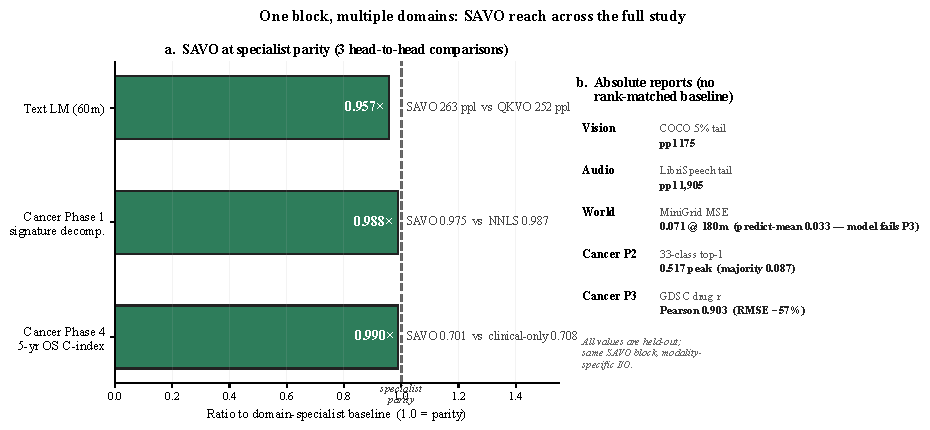
\includegraphics[width=.989\linewidth]{figs/fig18.pdf}
  \caption{\textbf{One block, multiple domains.} Left: three head-to-head ratios where SAVO has a comparable specialist baseline --- text vs.\ rank-matched QKVO at 60m, signature decomposition vs.\ NNLS, and 5-year survival vs.\ clinical-only ablation. All three sit within ${\sim}$5\% of the specialist baseline; in each case the specialist baseline is in fact slightly better (rank-matched MHA $-$12 ppl vs SAVO; NNLS +0.012 cosine vs SAVO; clinical-only AUROC +0.006 vs full fusion). The architectural claim is invariance of the block, not domain superiority. Right: absolute SAVO held-out numbers for vision, audio, world, and the two cancer tasks for which there is no rank-matched single-domain baseline at our scale.}
  \label{fig:18}
\end{figure}

\section{Conclusion}\label{sec:8}

We evaluated \QC{}~\cite{ref1} as a single routing primitive across text, vision, audio, world-state transition,
and four cross-field cancer-ML tasks at three parameter scales (60m, 120m, 180m). SAVO --- the
four-projection variant in which the $V$ projects state$\odot$action --- closes the SAO$\to$QKVO 60m text-LM
gap to a 4-seed paired difference of $+12.33 \pm 0.87$ ppl above the rank-matched controlled ablation
($p = 7.6 \times 10^{-4}$); a comparable ${\sim}$11--12-ppl gap holds at 120m and 180m (single seed each). The
rank-matched transformer baseline is a controlled ablation isolating the value-projection question, not
a comparison against full-rank attention. At matched 60m text-compute, joint four-modality training
reaches the same per-text-token loss as text-only training, and the property holds through 180m. The same
SAVO block, with no architectural changes, runs on signature decomposition (cosine 0.975 vs NNLS
0.987), 27-class pan-cancer classification (top-1 0.517), GDSC2 drug-response regression ($r = 0.903$),
and TCGA 5-year-survival prediction (C-index 0.701). The world-model branch trains stably as a fourth
concurrent objective (world MSE $1.125 \to 0.071$ over the training budget); MiniGrid-Empty-8x8's low
encoded next-state variance puts the predict-mean baseline (0.033) in the same band, so benchmarking
against dedicated world-model architectures on demanding environments (DMLab, Habitat) is left as
future work. \NanoG{} (cancer foundation model with mid-CoT hypothetical simulation, building on \S\ref{sec:7})
is the named successor project whose results will be reported separately.

\section*{Data and Code Availability}

All training scripts, dataset preparation scripts, figure-generation scripts, and checkpoints are released
under the MIT license at \url{https://github.com/Abd0r/quatrix}. All quantitative results in this paper
are reproducible from a clean checkout on a single 6\,GB consumer GPU. The arxiv + pubmed OOD
subsets used in \S\ref{sec:5.4} are reproducible from the data-preparation script. No human-subjects data were
collected by this work; the TCGA-CDR and GDSC2 data used in \S\ref{sec:7} are obtained from their public
release URLs.

\section*{AI Assistance Disclosure}

Claude (Anthropic) was used as a writing and coding assistant during preparation of this manuscript,
figure-generation scripts, and training pipeline. The author conceived the architecture, designed all
experiments, verified all results, and takes full responsibility for the scientific content.

\section*{Acknowledgments}

This work was conducted independently, without institutional affiliation or external funding.

\begin{thebibliography}{99}

\bibitem{ref1}
Syed Abdur Rehman Ali.
\newblock Q-Compass: Grounding sequence mixing in reinforcement learning navigation, March 2026.
\newblock URL \url{https://zenodo.org/records/19104202}.
\newblock Independent preprint.

\bibitem{ref2}
Alexey Dosovitskiy, Lucas Beyer, Alexander Kolesnikov, Dirk Weissenborn, Xiaohua Zhai, Thomas
  Unterthiner, Mostafa Dehghani, Matthias Minderer, Georg Heigold, Sylvain Gelly, Jakob Uszkoreit,
  and Neil Houlsby.
\newblock An image is worth 16x16 words: Transformers for image recognition at scale.
\newblock In \emph{International Conference on Learning Representations (ICLR)}, 2021.

\bibitem{ref3}
Alec Radford, Jong Wook Kim, Tao Xu, Greg Brockman, Christine McLeavey, and Ilya Sutskever.
\newblock Robust speech recognition via large-scale weak supervision.
\newblock In \emph{International Conference on Machine Learning (ICML)}, 2023.

\bibitem{ref4}
Alec Radford, Jeffrey Wu, Rewon Child, David Luan, Dario Amodei, and Ilya Sutskever.
\newblock Language models are unsupervised multitask learners.
\newblock \emph{OpenAI Technical Report}, 2019.

\bibitem{ref5}
Ashish Vaswani, Noam Shazeer, Niki Parmar, Jakob Uszkoreit, Llion Jones, Aidan N. Gomez,
  Lukasz Kaiser, and Illia Polosukhin.
\newblock Attention is all you need.
\newblock In \emph{Advances in Neural Information Processing Systems (NeurIPS)}, volume~30, 2017.

\bibitem{ref6}
Angelos Katharopoulos, Apoorv Vyas, Nikolaos Pappas, and Fran\c{c}ois Fleuret.
\newblock Transformers are RNNs: Fast autoregressive transformers with linear attention.
\newblock In \emph{International Conference on Machine Learning (ICML)}, 2020.

\bibitem{ref7}
Rewon Child, Scott Gray, Alec Radford, and Ilya Sutskever.
\newblock Generating long sequences with sparse transformers.
\newblock \emph{arXiv preprint arXiv:1904.10509}, 2019.

\bibitem{ref8}
Tri Dao, Daniel~Y. Fu, Stefano Ermon, Atri Rudra, and Christopher R\'{e}.
\newblock FlashAttention: Fast and memory-efficient exact attention with IO-awareness.
\newblock In \emph{Advances in Neural Information Processing Systems (NeurIPS)}, 2022.

\bibitem{ref9}
Joshua Ainslie, James Lee-Thorp, Michiel de~Jong, Yury Zemlyanskiy, Federico Lebr\'{o}n, and Sumit
  Sanghai.
\newblock GQA: Training generalized multi-query transformer models from multi-head checkpoints.
\newblock \emph{arXiv preprint arXiv:2305.13245}, 2023.

\bibitem{ref10}
Alec Radford, Jong Wook Kim, Chris Hallacy, Aditya Ramesh, Gabriel Goh, Sandhini Agarwal,
  Girish Sastry, Amanda Askell, Pamela Mishkin, Jack Clark, Gretchen Krueger, and Ilya Sutskever.
\newblock Learning transferable visual models from natural language supervision.
\newblock In \emph{International Conference on Machine Learning (ICML)}, 2021.

\bibitem{ref11}
Jean-Baptiste Alayrac, Jeff Donahue, Pauline Luc, Antoine Miech, Iain Barr, Yana Hasson, Karel
  Lenc, Arthur Mensch, Katie Millican, Malcolm Reynolds, Roman Ring, Eliza Rutherford, Serkan
  Cabi, Tengda Han, Zhitao Gong, Sina Samangooei, Marianne Monteiro, Jacob Menick, Sebastian
  Borgeaud, Andrew Brock, Aida Nematzadeh, Sahand Sharifzadeh, Mikolaj Binkowski, Ricardo
  Barreira, Oriol Vinyals, Andrew Zisserman, and Karen Simonyan.
\newblock Flamingo: A visual language model for few-shot learning.
\newblock In \emph{Advances in Neural Information Processing Systems (NeurIPS)}, 2022.

\bibitem{ref12}
Andrew Jaegle, Sebastian Borgeaud, Jean-Baptiste Alayrac, Carl Doersch, Catalin Ionescu, David
  Ding, Skanda Koppula, Daniel Zoran, Andrew Brock, Evan Shelhamer, Olivier H\'{e}naff, Matthew~M.
  Botvinick, Andrew Zisserman, Oriol Vinyals, and Jo\~{a}o Carreira.
\newblock Perceiver IO: A general architecture for structured inputs \& outputs.
\newblock In \emph{International Conference on Learning Representations (ICLR)}, 2022.

\bibitem{ref13}
Scott Reed, Konrad \.{Z}o\l{}na, Emilio Parisotto, Sergio G\'{o}mez Colmenarejo, Alexander Novikov,
  Gabriel Barth-Maron, Mai Gim\'{e}nez, Yury Sulsky, Jackie Kay, Jost Tobias Springenberg, Tom
  Eccles, Jake Bruce, Ali Razavi, Ashley Edwards, Nicolas Heess, Yutian Chen, Raia Hadsell, Oriol
  Vinyals, Mahyar Bordbar, and Nando de~Freitas.
\newblock A generalist agent.
\newblock \emph{Transactions on Machine Learning Research (TMLR)}, 2022.

\bibitem{ref14}
David Ha and J\"{u}rgen Schmidhuber.
\newblock Recurrent world models facilitate policy evolution.
\newblock In \emph{Advances in Neural Information Processing Systems (NeurIPS)}, 2018.

\bibitem{ref15}
Danijar Hafner, Jurgis Pasukonis, Jimmy Ba, and Timothy Lillicrap.
\newblock Mastering diverse domains through world models.
\newblock \emph{arXiv preprint arXiv:2301.04104}, 2023.

\bibitem{ref16}
Keller Jordan.
\newblock Muon: An optimizer for the hidden layers of neural networks.
\newblock \url{https://kellerjordan.github.io/posts/muon/}, 2024.

\bibitem{ref17}
Ilya Loshchilov and Frank Hutter.
\newblock Decoupled weight decay regularization.
\newblock In \emph{International Conference on Learning Representations (ICLR)}, 2019.

\bibitem{ref18}
DeepSeek-AI.
\newblock Deepseek-v4: Towards highly efficient million-token context intelligence.
\newblock \emph{arXiv preprint}, 2026.
\newblock Preview release. Model checkpoints: \url{https://huggingface.co/collections/deepseek-ai/deepseek-v4}.

\bibitem{ref19}
Stephen Merity, Caiming Xiong, James Bradbury, and Richard Socher.
\newblock Pointer sentinel mixture models.
\newblock In \emph{International Conference on Learning Representations (ICLR)}, 2017.

\bibitem{ref20}
Tsung-Yi Lin, Michael Maire, Serge Belongie, James Hays, Pietro Perona, Deva Ramanan, Piotr
  Doll\'{a}r, and C.~Lawrence Zitnick.
\newblock Microsoft COCO: Common objects in context.
\newblock In \emph{European Conference on Computer Vision (ECCV)}, 2014.

\bibitem{ref21}
Vassil Panayotov, Guoguo Chen, Daniel Povey, and Sanjeev Khudanpur.
\newblock LibriSpeech: An ASR corpus based on public domain audio books.
\newblock In \emph{IEEE International Conference on Acoustics, Speech and Signal Processing (ICASSP)}, 2015.

\bibitem{ref22}
Maxime Chevalier-Boisvert, Bolun Dai, Mark Towers, Rodrigo de~Lazcano, Lucas Willems, Salem
  Lahlou, Suman Pal, Pablo~Samuel Castro, and Jordan Terry.
\newblock Minigrid \& miniworld: Modular \& customizable reinforcement learning environments for
  goal-oriented tasks.
\newblock \url{https://github.com/Farama-Foundation/Minigrid}, 2023.
\newblock Gymnasium compatible RL benchmark.

\bibitem{ref23}
DeepSeek-AI.
\newblock Deepseek-v2: A strong, economical, and efficient mixture-of-experts language model.
\newblock \emph{arXiv preprint arXiv:2405.04434}, 2024.

\bibitem{ref24}
Noam Shazeer.
\newblock Fast transformer decoding: One write-head is all you need.
\newblock \emph{arXiv preprint arXiv:1911.02150}, 2019.

\bibitem{ref25}
Edward~J. Hu, Yelong Shen, Phillip Wallis, Zeyuan Allen-Zhu, Yuanzhi Li, Shean Wang, Lu~Wang,
  and Weizhu Chen.
\newblock LoRA: Low-rank adaptation of large language models.
\newblock In \emph{International Conference on Learning Representations (ICLR)}, 2022.

\bibitem{ref26}
Sinong Wang, Belinda~Z. Li, Madian Khabsa, Han Fang, and Hao Ma.
\newblock Linformer: Self-attention with linear complexity.
\newblock \emph{arXiv preprint arXiv:2006.04768}, 2020.

\bibitem{ref27}
Krzysztof Choromanski, Valerii Likhosherstov, David Dohan, Xingyou Song, Andreea Gane,
  Tamas Sarlos, Peter Hawkins, Jared Davis, Afroz Mohiuddin, Lukasz Kaiser, David Belanger, Lucy
  Colwell, and Adrian Weller.
\newblock Rethinking attention with Performers.
\newblock In \emph{International Conference on Learning Representations (ICLR)}, 2021.

\bibitem{ref28}
Ludmil~B. Alexandrov, Jaegil Kim, Nicholas~J. Haradhvala, Mi~Ni Huang, Alvin~W. Tian~Ng, Yang
  Wu, Arnoud Boot, Kyle~R. Covington, Dmitry~A. Gordenin, Erik~N. Bergstrom, S.~M. Ashiqul
  Islam, et~al.
\newblock The repertoire of mutational signatures in human cancer.
\newblock \emph{Nature}, 578:94--101, 2020.

\bibitem{ref29}
S.~M. Ashiqul Islam, Marcos D\'{i}az-Gay, Yang Wu, Mark Barnes, Raviteja Vangara, Erik~N.
  Bergstrom, Yudou He, Mike Vella, Jingwei Wang, Jon~W. Teague, Peter Clapham, et~al.
\newblock Uncovering novel mutational signatures by de novo extraction with SigProfilerExtractor.
\newblock \emph{Cell Genomics}, 2(11):100179, 2022.

\bibitem{ref30}
Kyle Ellrott, Matthew~H. Bailey, Gordon Saksena, Kyle~R. Covington, Cyriac Kandoth, Chip
  Stewart, Julian Hess, Singer Ma, Kami~E. Chiotti, Michael McLellan, et~al.
\newblock Scalable open science approach for mutation calling of tumor exomes using multiple genomic
  pipelines (MC3).
\newblock \emph{Cell Systems}, 6(3):271--281.e7, 2018.

\bibitem{ref31}
Wanjuan Yang, Jorge Soares, Patricia Greninger, Elena~J. Edelman, Howard Lightfoot, Simon
  Forbes, Nidhi Bindal, Dave Beare, James~A. Smith, I.~Richard Thompson, et~al.
\newblock Genomics of drug sensitivity in cancer (GDSC): a resource for therapeutic biomarker
  discovery in cancer cells.
\newblock \emph{Nucleic Acids Research}, 41(D1):D955--D961, 2013.

\bibitem{ref32}
Jianfang Liu, Tara Lichtenberg, Katherine~A. Hoadley, Laila~M. Poisson, Alexander~J. Lazar,
  Andrew~D. Cherniack, Albert~J. Kovatich, Christopher~C. Benz, Douglas~A. Levine, Adrian~V. Lee,
  et~al.
\newblock An integrated TCGA pan-cancer clinical data resource to drive high-quality survival outcome
  analytics.
\newblock \emph{Cell}, 173(2):400--416.e11, 2018.

\end{thebibliography}


\end{document}
